% This is samplepaper.tex, a sample chapter demonstrating the
% LLNCS macro package for Springer Computer Science proceedings;
% Version 2.20 of 2017/10/04
%
\documentclass[runningheads,final]{llncs}
%
\usepackage{hyperref}
\usepackage{multicol}
\usepackage[final]{changes}
\usepackage{url}
\usepackage{amsmath}
\usepackage{bm}
\usepackage{multirow}
\usepackage{tcolorbox}
\usepackage{rotating}
\usepackage{latexsym,amssymb,amsmath}
\usepackage{makecell}
\usepackage{xspace}
\usepackage{paralist}
\usepackage{wrapfig}
\usepackage{adjustbox}
%%%%%%%%%%%%%%%%%%%%%%%%%%%%%%%%%%%%%%%%%%%%%%%%%%%%%%%%%%%%%%%%%%%%%%%%%%%%%%
%%% Time-stamp: "2018-09-07 18:35:03 calvanese"
%%%%%%%%%%%%%%%%%%%%%%%%%%%%%%%%%%%%%%%%%%%%%%%%%%%%%%%%%%%%%%%%%%%%%%%%%%%%%%

%%%%%%%%%%%%%%%%%%%%%%%%%% General Math

\newcommand{\A}{\ensuremath{\mathcal{A}}}
\newcommand{\B}{\ensuremath{\mathcal{B}}}
%\newcommand{\C}{\ensuremath{\mathcal{C}}}
\newcommand{\D}{\ensuremath{\mathcal{D}}}
\newcommand{\E}{\ensuremath{\mathcal{E}}}
\newcommand{\F}{\ensuremath{\mathcal{F}}}
%\newcommand{\G}{\ensuremath{\mathcal{G}}}
\renewcommand{\H}{\ensuremath{\mathcal{H}}}
\newcommand{\I}{\ensuremath{\mathcal{I}}}
\newcommand{\J}{\ensuremath{\mathcal{J}}}
\newcommand{\K}{\ensuremath{\mathcal{K}}}
\renewcommand{\L}{\ensuremath{\mathcal{L}}}
\newcommand{\M}{\ensuremath{\mathcal{M}}}
\newcommand{\N}{\ensuremath{\mathcal{N}}}
\renewcommand{\O}{\ensuremath{\mathcal{O}}}
\renewcommand{\P}{\ensuremath{\mathcal{P}}}
\newcommand{\Q}{\ensuremath{\mathcal{Q}}}
\newcommand{\R}{\ensuremath{\mathcal{R}}}
%\renewcommand{\S}{\ensuremath{\mathcal{S}}}
\newcommand{\T}{\ensuremath{\mathcal{T}}}
%\newcommand{\U}{\ensuremath{\mathcal{U}}}
\newcommand{\V}{\ensuremath{\mathcal{V}}}
\newcommand{\W}{\ensuremath{\mathcal{W}}}
\newcommand{\X}{\ensuremath{\mathcal{X}}}
\newcommand{\Y}{\ensuremath{\mathcal{Y}}}
\newcommand{\Z}{\ensuremath{\mathcal{Z}}}

%%%%%%%%%%%%%%%%%%%%%%%%%% Abbreviations

%%\newcommand{\eset}{\emptyset}
%%\newcommand{\col}{\colon}
\newcommand{\ol}[1]{\overline{#1}}                % overline
%\newcommand{\ul}[1]{\underline{#1}}               % underline
%%\newcommand{\uls}[1]{\underline{\raisebox{0pt}[0pt][0.45ex]{}#1}}
%% ul with space between text and line

\newcommand{\ra}{\rightarrow}
\newcommand{\Ra}{\Rightarrow}
\newcommand{\la}{\leftarrow}
\newcommand{\La}{\Leftarrow}
%\newcommand{\lra}{\leftrightarrow}
\newcommand{\Lra}{\Leftrightarrow}
\newcommand{\lora}{\longrightarrow}
\newcommand{\Lora}{\Longrightarrow}
\newcommand{\lola}{\longleftarrow}
\newcommand{\Lola}{\Longleftarrow}
\newcommand{\lolra}{\longleftrightarrow}
\newcommand{\Lolra}{\Longleftrightarrow}
%\newcommand{\ua}{\uparrow}
\newcommand{\Ua}{\Uparrow}
\newcommand{\da}{\downarrow}
\newcommand{\Da}{\Downarrow}
\newcommand{\uda}{\updownarrow}
\newcommand{\Uda}{\Updownarrow}

%%%%%%%%%%%%%%%%%%%%%%%%%% Relations

%%\newcommand{\incl}{\subseteq}
%%\newcommand{\imp}{\rightarrow}
\newcommand{\per}{\mbox{\bf .}}                  % period

%%%%%%%%%%%%%%%%%%%%%%%%%% Delimiters

%%\newcommand{\quotes}[1]{{\lq\lq #1\rq\rq}}
%\newcommand{\set}[1]{\{#1\}}                      % set
%\newcommand{\Set}[1]{\left\{#1\right\}}
\newcommand{\bigset}[1]{\Bigl\{#1\Bigr\}}
\newcommand{\bigmid}{\Big|}
\newcommand{\size}[1]{|{#1}|}                     % cardinality of a set
%%\newcommand{\Card}[1]{\left| #1\right|}
\newcommand{\card}[1]{\sharp #1}
\newcommand{\tup}[1]{\langle #1\rangle}            % tuple
\newcommand{\Tup}[1]{\Braket{#1}}
\newcommand{\norm}[2]{\|#1\|_{#2}}
\newcommand{\setone}[2][1]{\set{#1\cld #2}}

%%%%%%%%%%%%%%%%%%%%%%%%%% STYLING AND SPACING

%\newcommand{\inlinetitle}[1]{\smallskip\noindent\textbf{#1.}\xspace}





\newcolumntype{C}{>{\centering\arraybackslash}X}

%\makeatletter
%\g@addto@macro\normalsize{%
%\setlength{\abovecaptionskip}{-2pt}
%\setlength{\belowcaptionskip}{12pt}
%\setlength\abovedisplayskip{3pt}
%\setlength\belowdisplayskip{3pt}
%\setlength\abovedisplayshortskip{3pt}
%\setlength\belowdisplayshortskip{3pt}
%}
%\makeatother

\newcounter{dummy} 
\newcounter{dummy1} 
\newcounter{dummy2}
\newcounter{dummy3} 
\newcounter{dummy4}
\newcounter{dummy5} 
\newcounter{dummy6}
\newcounter{dummy7}
%\numberwithin{dummy}{section}

\usepackage[thmmarks,amsmath]{ntheorem}
%\theorempreskip{1pt}
%\theorempostskip{1pt}

%\theoremstyle{plain}
%\theorembodyfont{\normalfont}
%\theoremseparator{.}
%\let\definition\relax
%\theoremsymbol{\ensuremath{\square}}
%\newtheorem{definition}{Definition}


\let\proposition\relax
\let\theorem\relax
\let\lemma\relax
\let\definition\relax
\theoremseparator{.}
\theorembodyfont{\itshape}
\theoremsymbol{$\triangleleft$}
\newtheorem{theorem}[dummy]{Theorem}
\newtheorem{lemma}[dummy1]{Lemma}
\newtheorem{definition}[dummy2]{Definition}
\newtheorem{proposition}[dummy3]{Proposition}

\let\remark\relax
\let\example\relax
%\let\example*\relax
\theorembodyfont{\normalfont}
\newtheorem{example}[dummy4]{Example}
\newtheorem{remark}[dummy5]{Remark}
%\newtheorem{example*}[dummy4]{Example}


\theoremstyle{nonumberplain}
\theoremheaderfont{\itshape}
\theorembodyfont{\normalfont}
\let\proof\relax
\theoremseparator{.}
\theoremsymbol{\ensuremath{\dashv}}
\newtheorem{proof}[dummy6]{Proof}


\qedsymbol{\ensuremath{\dashv}}


%%% Local Variables:
%%% mode: latex
%%% TeX-master: "main"
%%% save-place: t
%%% End:



\usepackage{graphicx}
\usepackage{xcolor,color}
\usepackage{subfig}
\usepackage{tikz}
\usepackage{calc}

\usepackage{tabularx}
\usepackage{booktabs}

\usepackage{ulem}

\usepackage{kbordermatrix}
\usepackage{amsmath,amsfonts}
\usepackage{braket}
\usepackage{xfrac}

\usepackage{pifont}
\usepackage{amssymb}
\usepackage{paralist}
\usepackage[inline]{enumitem}

\usepackage{varioref}
\newcommand{\pmin}{\rho}

\newcommand{\const}[1]{\mathsf{#1}}

\newcommand{\alphabet}{\Sigma}
\newcommand{\tasks}{\mathcal{A}}
\newcommand{\hidden}{\tau}

\newcommand{\uswn}{SWN\xspace}
\newcommand{\net}{\ensuremath{N}}
\newcommand{\tg}{\ensuremath{G}}
\newcommand{\closed}[1]{\overline{#1}}
\newcommand{\marking}{m}
\newcommand{\enaset}[2]{E_{#2}(#1)}
\newcommand{\fire}[4]{#1\xrightarrow{#2}_{#4}#3}
\newcommand{\probt}[3]{\mathbb{P}_{#2,#3}(#1)}
\newcommand{\prob}[2]{\mathbb{P}_{#2}(#1)}
\newcommand{\rg}[1]{RG(#1)}
\newcommand{\ind}[1]{\textnormal{\texttt{#1}}}
\newcommand{\seq}{\eta}
\newcommand{\run}{\xi}
\newcommand{\trace}{\sigma}
\newcommand{\traces}[1]{\mathit{traces}(#1)}
\newcommand{\ptraces}[2]{\mathit{ptraces}_{#2}(#1)}

\newcommand{\nreach}[3][]{#2 \overset{#1}{\rightsquigarrow} #3}
\newcommand{\runs}[2]{runs_{#2}(#1)}
\newcommand{\seqs}[2]{seqs_{#2}(#1)}
\newcommand{\transp}[1]{#1^\top}
\newcommand{\embed}{\phi}
\newcommand{\trembed}{\embed^{\text{tr}}}
\newcommand{\gorgembed}{\embed^{g}}


\newcommand{\pa}{\rho_{23}}
\newcommand{\pb}{\rho_{24}}
\newcommand{\pc}{\rho_{55}}
\newcommand{\pd}{\rho_{65}}
\newcommand{\pe}{\rho_{67}}
\newcommand{\pf}{\rho_{57}}

\newcommand{\logtrace}{\trace}
\newcommand{\nonlogtrace}{{\trace'}}


\newcommand{\approptoinn}[2]{\mathrel{\vcenter{
			\offinterlineskip\halign{\hfil$##$\cr
				#1\propto\cr\noalign{\kern2pt}#1\sim\cr\noalign{\kern-2pt}}}}}
\newcommand{\appropto}{\mathpalette\approptoinn\relax}


\newcommand{\unravelled}{unfolded}
\newcommand{\unravelling}{unfolding}
\newcommand{\unravel}{unfold}



%
%\def\WWITHN{def}
%\ifdefined\WWITHN
%\newcommand{\WCal}[2]{{\mathcal{W}_{#1}^{#2}}}
%\newcommand{\TBf}[2]{{\mathbf{T}_{#1}^{#2}}}
%\else
\newcommand{\TBf}[2]{{\mathbf{G}_{#1}}}
%\fi
\newcommand{\expN}{\closed{\tg_{\rg{\net}}}}

\def\EqualityHolds{itholds}
\ifdefined\EqualityHolds
\newcommand{\probarg}{\net}
\newcommand{\WCal}[2]{\ptraces{\net}{#1}}
\else
\newcommand{\probarg}{\expN}
\newcommand{\WCal}[2]{\ptraces{\closed{\tg_{\rg{\net}}}}{#1}}
\fi
\newcommand{\probskip}[1]{\prob{#1}{\probarg}}
\newcommand{\goldenrank}{\mathcal{R}} 


\begin{document}

%
\title{Probabilistic Trace Alignment}
%\subtitle{\emph{Vision Paper}}
%
%\titlerunning{Abbreviated paper title}
% If the paper title is too long for the running head, you can set
% an abbreviated paper title here
%
\author{
	Giacomo Bergami\inst{1} \and
	Fabrizio Maria Maggi\inst{1} \and
	Marco Montali\inst{1} \and
	Rafael Pe\~naloza\inst{2}}

\authorrunning{G.~Bergami, F.M.~Maggi, M.~Montali and R.~Pe\~naloza}
% First names are abbreviated in the running head.
% If there are more than two authors, 'et al.' is used.
%
\institute{
	Free University of Bozen-Bolzano, Italy \\\email{gibergami@unibz.it,\{maggi,montali\}@inf.unibz.it}
	\and
	University of Milano-Bicocca \\\email{rafael.penaloza@unimib.it}
}

%\vspace{1.5cm}
%
%
\maketitle              % typeset the header of the contribution
%\linespread{0.98}
%\vspace{-0.5cm}

\begin{abstract}
Conformance checking techniques verify whether the observed behavior recorded in an event log matches a modeled behavior. This type of analysis is crucial, because often real process executions deviate from the reference process models. In the existing literature on conformance checking, one of the most common approaches is based on trace alignments. Alignments provide sophisticated diagnostics that pinpoint where deviations occur in a trace with respect to a process model and how severe they are. However, the proposed approaches based on trace alignments use crisp process models as reference models. On the other hand, recently, probabilistic conformance checking approaches are gaining momentum, but the existing approaches are used to check the degree of conformance of an event log with respect to a stochastic process model instead of finding trace alignments.
In this paper, for the first time, we provide a conformance checking approach based on trace alignments using a stochastic Petri net. Conceptually, this requires to handle the two possibly contrasting forces of the cost of the alignment on the one hand and the likelihood of the model trace with respect to which the alignment is computed on the other. If the cost of the alignment is too high, even if the considered model trace is very likely, applying too many changes in the original trace is not always the best option. The approach has been evaluated using both synthetic and real-life logs.
\end{abstract}

\keywords{Declarative Process Models, Probabilistic Temporal Logics, Conformance Checking}

%

% !TeX root=../main.tex

\section{Introduction}
\label{introduction}
%Trace alignment is a well-known technique in conformance checking \cite{DBLP:conf/edoc/AdriansyahDA11} providing both a numerical assessment of the degree of conformance of a log trace with respect to a model, as well as a repair strategy if such trace does not conform to the given model. At the time of the writing,
%
In the existing literature on conformance checking, a common approach is based on trace alignment \cite{DBLP:conf/edoc/AdriansyahDA11}. This approach uses crisp process models as reference models. Yet, recently developed probabilistic conformance checking approaches provide a numerical quantification of the degree of conformance
%the existing approaches are used to check the degree of conformance
of an event log with a stochastic process model by either assessing the distribution discrepancies \cite{DBLP:conf/bpm/LeemansSA19}, or by exploiting entropy-based measures \cite{DBLP:conf/icpm/PolyvyanyyK19,DBLP:journals/tosem/PolyvyanyySWCM20}.
As these strategies are not based on trace alignments, these cannot be directly used to repair a given trace with one of the traces generated by a stochastic process model.
%As traces generated by such models are associated to a probability exhibiting its representativeness and relevance within the model, probabilistic trace alignment techniques should take into account the combined provision of trace probability and alignment cost.
%instead of finding trace alignments.

In this paper, we provide for the first time an approach for the probabilistic alignment of a trace and a stochastic reference
model. This approach is not comparable with the existing literature on probabilistic conformance checking as its output is not numeric but consists of a ranked list of alignments.
Providing different alignment options is useful since, conceptually, probabilistic trace alignment requires the analyst to 
%handle the two possibly contrasting forces of the cost of the alignment on the one hand and the likelihood of the model trace with respect to which the alignment is computed.
%We consider the important tradeoff between both
%aspects.
balance between the likelihood of the model trace with respect to which the alignment is computed and the cost of the alignment. 
%(if the cost of the alignment is too high even if the model trace is very likely applying too many changes in the original trace is in turn not very likely).

\begin{figure}[!t]
	\centering
	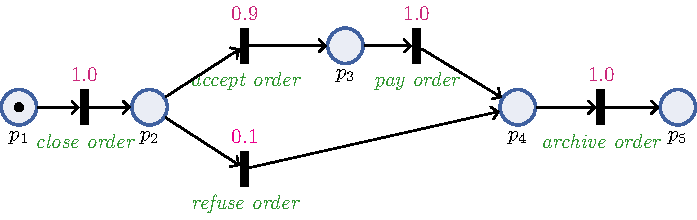
\includegraphics[width=.45\textwidth]{images/petri_tut.pdf}
	\caption{Stochastic Workflow Net modeling our use-case scenario.}\label{fig:petri_tut}
%\vspace{-0.6cm}
\end{figure}
%For example, the probabilistic alignment of a trace with a stochastic net could be represented by the model trace maximizing the combined provision of minimum trace alignment cost and maximum model trace probability. 
With reference to Figure~\ref{fig:petri_tut}, a user might be interested to align the log trace $\langle \textsf{close order},\,\textsf{archive order}\rangle$ with one of the two possible model traces $\langle\textsf{close order},$ $\textsf{accept order},\,\textsf{pay order},\,\textsf{archive order}\rangle$ or $\langle$\textsf{close order}, \textsf{refuse order}, \textsf{archive order}$\rangle$. While the latter trace provides the least alignment cost though the model trace has a low probability ($0.1$), the former gives a slightly greater alignment cost while providing a higher model trace probability ($0.9$). Since, depending on the context, analysts might prefer either the former or the latter alignment, providing a selection of the best $k$ alignments among all the distinct model traces empowers the analysts to find their own trade-off between alignment cost and model trace probability.
%However, in some cases, the user could prefer to identify an alignment with a lower cost even if based on a less probable model trace, while, in other cases, the user could favor a model trace with a higher probability at the expense of a higher alignment cost. Therefore, to provide users with an instrument that allows them to find their own trade-off between alignment cost and model trace probability, we need to return the best $k$ alignments among all the distinct model traces.
%Since when aligning an event log with a stochastic net distinct model traces have different probabilities, the retrieval of the best model trace maximizing the combined provision of minimum trace alignment cost and maximum model trace probability might not suffice. In some cases, indeed, the user could prefer to identify an alignment with a lower cost even if based on a less probable model trace, while, in other cases, the user could favor a model trace with a higher probability at the expense of a higher alignment cost. We consider, therefore, the important tradeoff between both aspects.
%Therefore, in this paper, we propose trace alignment approaches that return the best
To do this, we frame the probabilistic trace alignment problem into the well-known $k$-Nearest Neighbors ($k$NN) problem \cite{Altman} that refers to finding the $k$ nearest data points to a \textit{query} $x$ from a set $\mathcal{X}$ of \textit{data points} via a distance function defined over $\mathcal{X}\cup\{x\}$.
We introduce two ranking strategies. The first one is based on a brute force approach that reuses existing trace aligners  \cite{DBLP:conf/edoc/AdriansyahDA11,LeoniM17} %, where the (optimal) ranking of the top-k alignments is obtained by computing the Levensthein distance between the trace to be aligned and all the model traces and by multiplying each of these distances by the probability of the corresponding model trace. However, even if this approach returns the best trace alignment ranking for a query trace,
requiring to re-compute
 the alignments %must be computed a-new 
 for all the possible traces.% to be aligned. 
 For models generating a large number of model traces, this would clearly become unfeasible: % Therefore, we propose a
 the 
 second strategy %that
  produces an approximate ranking where $x$ and $\mathcal{X}$ are represented as numerical vectors via an embedding $\phi$. 
  %{Then, by exploiting ad-hoc data structures,
%such as Vp-Trees \cite{Fu2000}, Kd-Trees \cite{Maneewongvatana99}, and M-Trees \cite{Ciaccia},
%we can retrieve the neighborhood of $x$ in $\mathcal{X}$ of size $k$  by pre-ordering (\textit{indexing}) $\mathcal{X}$  via a distance between the numerical vectors obtained using $\phi$. 
%Thus, we do not need to analyze the entire space, but just start the search from the top-$1$ alignment. 
If the embeddings $\phi$ for $\mathcal{X}$ are independent of the query of choice $x$, this would not require to constantly recompute the numeric vector representation for $\mathcal{X}$ and to pre-order $\mathcal{X}$ to efficiently visit the search space.
%	
%%%%% Proposed part as the last part of the introduction:
%\texttt{\color{red}[TODO]}
%\todo{this is too specific for an introduction; in particular, too many details on how the experiments are done.}
%We implemented both strategies and perform experiments using a real life event log coming from a hospital system to empirically evaluate the properties of our proposed  strategy. Specifically, we (i) evaluate the correlation between the approximate rankings (using different ways for computing the embeddings) and the optimal ranking, and (ii)~compare the computation time for the exact trace alignment approach against the embedding-based approach. We show that the approximate ranking strategy exploiting a specific data structure (KD-Trees) provides the best trade-off between approximation and execution time, while being more efficient than both the exact ranking and the same approximate ranking with a different data structure (VP-Trees).
%In the next section, we describe the steps required by the tool to compute both alignment strategies. After briefly discussing some preliminary benchmarks, we propose some future work.
\begin{figure}[!t]
	\centering
	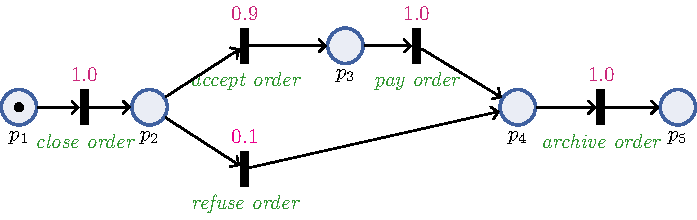
\includegraphics[width=.49\textwidth]{images/petri_tut.pdf}
	\caption{Stochastic Workflow Net modeling our use-case scenario.}\label{fig:petri_tut}
\end{figure}
\begin{figure}[!t]
	\centering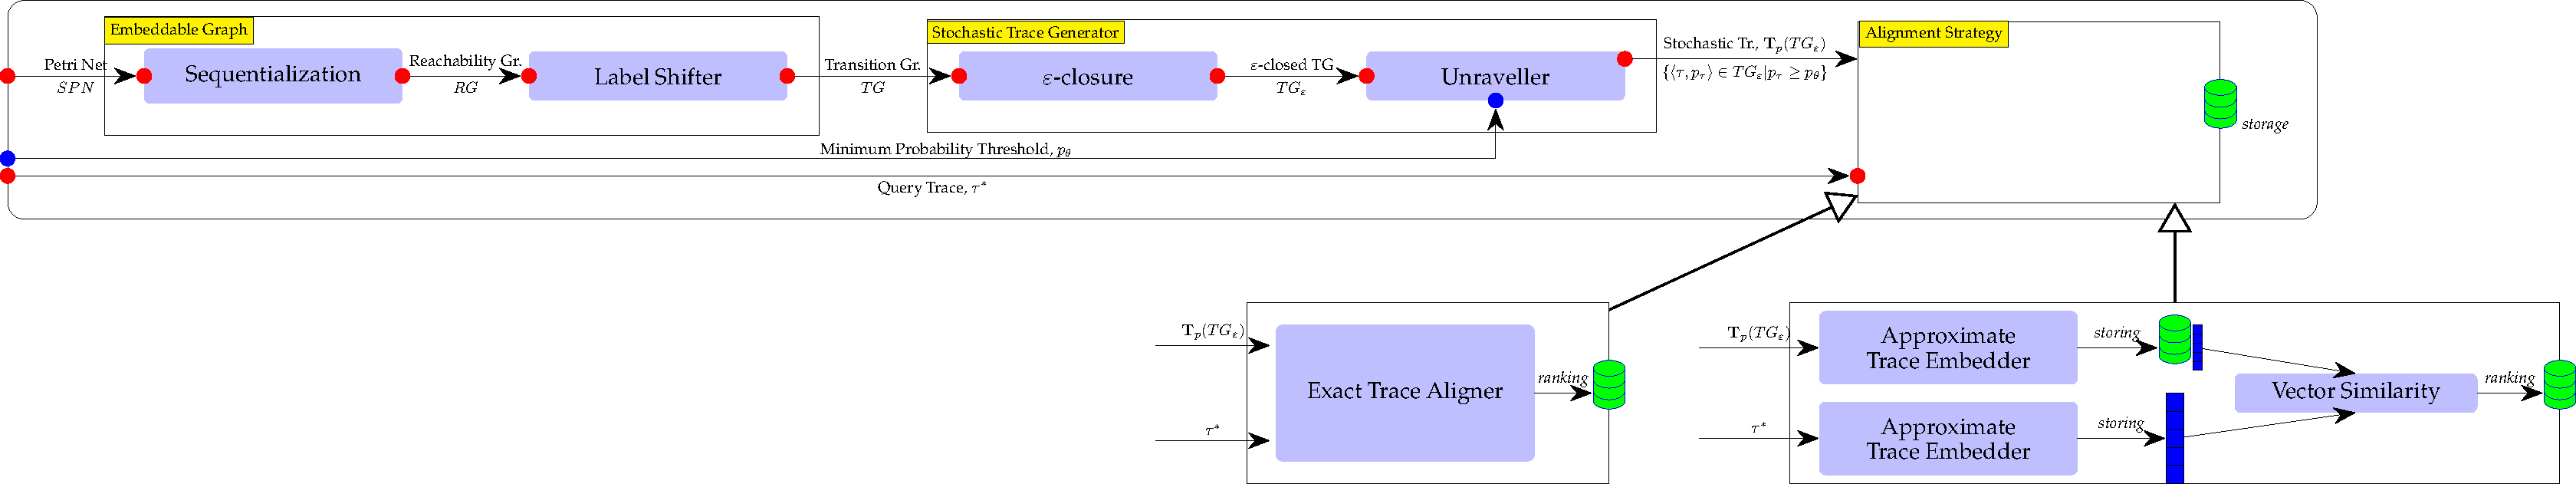
\includegraphics[width=.7\textwidth]{images/pipeline}
	\caption{Proposed pipeline to assess the probabilistic trace alignment.}\label{fig:pipe}
	\vspace*{-0.5cm}
\end{figure}

\section{Probabilistic Trace Alignment Pipeline}
%We now describe the proposed technique for computing probabilistic trace alignments. 
Our approach (\figurename~\ref{fig:pipe}) takes as input
\begin{inparaenum}[\it (i)]
	\item a reference model represented as an Stochastic Workflow Nets $\net$ or an equivalent Transition Graph $G$,
	\item a minimum, positive probability threshold $\pmin \in (0,1]$
	\item a trace $\trace$ of interest,
\end{inparaenum}
and returns a ranking over all the $\net$-traces having a probability greater than or equal to $\pmin$, based on a combined consideration of their probability values and their distance to $\trace$. First, we discuss input formats for \textit{(i)} as in the GUI.


%\section{Modeling Probabilistic Dynamic Systems}
%\label{sec:models}
%In this section, we introduce the different models and techniques that will constitute the basis for representing and computing probabilistic trace alignments.


%\subsection{Input}
%\subsection{Stochastic Workflow Nets}\label{subsec:spn}

\textbf{{Format: \texttt{Petri\_PNML}}.} Petri Nets and Generalized Stochastic Petri Nets are well-established formalisms \cite{DBLP:journals/tosem/PolyvyanyySWCM20} for modelling processes \cite{RoggeSoltiAW13} represented in the Petri Net Markup Language, supported by our tool. Due to the lack of space, we refer to \cite{spdwe} for the usual notation over Petri Nets. We restrict our interest to an interesting class of $1$-\textit{bounded} stochastic Petri nets with no timed transitions, namely \textsc{untimed Stochastic Workflow Nets} denoted as $N$. We now sketch the properties of the SWN accepted in PNML format and loaded as \textsf{PetriNet} objects: we consider two customary markings: the \emph{input} (resp.~\emph{output}) marking $m_{in}$ (resp.~$m_{out}$) assigning a single token to the input (resp.~output) place, and no token elsewhere. We assume to have a set $\alphabet = \tasks \cup \set{\tau}$ of labels, where labels in $\tasks$ indicate process tasks, whereas $\tau$ indicates an invisible execution step ($\tau$-transition). Labels are associated to transitions via a labelling function $\lambda$. A \emph{trace} is a finite sequence of labels from $\tasks$.
%\begin{definition} An \emph{untimed Stochastic Workflow Net (\uswn)}
%	is a tuple $\net = (P,T,F,\ell,W)$ where:
%	\begin{inparaenum}[\itshape (i)]
%		%\begin{inparaenum}
%		\item $(P,T,F)$ is a standard \emph{Workflow net} with places $P$, transitions $T$, and flow relation $F$ such that there is exactly one \emph{input place} with no incoming arc, and exactly one \emph{output place} with no outgoing arcs;
%		\item $\ell: T \rightarrow \alphabet$ is a \emph{labeling function} mapping each transition $t \in T$ into a label $\ell(t) \in \alphabet$ - this either indicates the task executed upon firing $t$, or the fact that $t$ is an invisible transition (in the latter case, $\ell(t) = \tau$);
%		\item $W\colon T\to \mathbb{R}^+$ is a \emph{weight function} assigning a positive firing weight to each transition of the net.
%	\end{inparaenum}
%\end{definition}
%Given an \uswn $\net$, we use dot notation to extract its constitutive components (e.g., $\net.P$ denotes its places). \emph{The same dot notation will be used for the other structures introduced in the paper}. We also use $\net.in$ and $\net.out$ to respectively denote the input and output place of $\net$.
The current state of execution is captured by a marking, i.e., a multiset of places $P$ indicating how many tokens populate each place.
%As pointed out above, \emph{we always assume, as customary in BPM, that the input \uswn is \underline{bounded}}, that is, in every state the number of tokens associated to each place cannot exceed a maximum, fixed threshold.
The notions of transition enablement and firing are also the standard ones  \cite{MarsanCB84}: %, which provides the basis for capturing the stochastic behavior of the net. 
%We use the following notation: given a marking $\marking$ over \uswn $\net$,  $\enaset{\marking}{\net}$ is the set of enabled transitions in $\marking$; given transition $t \in \enaset{\marking}{\net}$, we write $\fire{\marking}{t}{\marking'}{\net}$ to capture the fact that, with, firing $t$ in $\marking$ results in the new marking $\marking'$. A \emph{firing sequence starting from marking $\marking_0$} is a sequence $t_1\cdots t_n$ of transitions from $\net.T$ so that, for every $i \in \set{1,\ldots,n}$, we have that $\fire{\marking_{i-1}}{t_i}{\marking_{i}}{\net}$. We say that the firing sequence results in $\marking_{n}$.
%
given a marking $\marking$ %of $N$ 
and an enabled transition $t \in T_e$, the \emph{firing probability} of $t$ in $\marking$ is $\probt{t}{\marking}{\net} = \frac{W(t)}{\sum_{t'\in T_e}W(t')}$. %As required, 
The probabilities associated to all enabled transitions in a marking always add up to 1.
 A \emph{valid sequence} $\seq = t_1\cdots t_n$ is a firing sequence starting from $m_{in}^\net$ and resulting in $m_{out}$. The probability $\prob{\seq}{\net}$ of a valid sequence is the product of the probabilities associated to each transition: $\prob{\seq}{\net} = \prod_{i \in \set{1,\ldots,n}}\prob{t_i}{\marking_{i-1},\net}$. % A sequence of labels $\run = \alpha_1 \cdots \alpha_n$ from $\alphabet$ is a \emph{run} if there exists a valid underlying sequence $\seq = t_1\cdots t_n$  having $\alpha_i$ as a label for each $t_i\in \seq$. Run $\run$ may have different underlying valid sequences in $\seqs{\run}{\net}$.
  A trace $\trace=\const{a}_1\cdots \const{a}_m$ is a \emph{model trace} (or $\net$-trace for short) if there exists a valid sequence $\seq = t_1\cdots t_n$ where the appended labels $\lambda(t_1)\cdots \lambda(t_n)$ is equivalent to $\trace$ once all the $\tau$-s are stripped.
  %underlying run $\run$ corresponding to $\trace$ once all $\tau$ are removed. 
  There may be multiple valide sequences $\seq\in\seqs{\trace}{\net}$ %$\runs{\trace}{\net}$ 
  underlying an $\net$-trace $\trace$. 
   $\traces{\net}$ is the (possibly infinite) set of $\net$-traces. For a trace $\trace$ of $\net$, its probability $\prob{\trace}{\net}$ is then obtained by collecting all its underlying runs, in turn collecting all their underlying valid sequences, and summing up their respective probabilities: $\prob{\trace}{\net} = %\sum_{\run \in \runs{\trace}{\net}} 
   \sum_{\seq \in \seqs{\trace}{\net}} \prob{\seq}{\net}$. This corresponds to the intuition that, to observe $\trace$, one can equivalently pick any of its underlying valid sequences. Notably, if a trace is not an $\net$-trace (i.e., it does not conform with $\net$), then its probability is 0.
 These structural properties makes them suitable for loading BPMN nets as well: when the \texttt{Petri\_BPMN} is choosen, either the firing weight estimator is constant by default (\texttt{W\_CONSTANT}), or we can choose one from \cite{spdwe}. 
\begin{example} %\small
\label{ex:net}
\figurename~\ref{fig:spn} shows an example of an \uswn with input place $p_1$ and output place $p_7$. One run of the net is $\const{\tau c \tau a a \tau}$, which corresponds to trace $\const{caa}$. Overall, the net supports infinitely many finite traces of the form (represented using regular expressions):
\begin{inparaenum}[\it (i)]
\item $\const{aa^*}$,
\item $\const{cb}$,
\item $\const{caa^*}$.
\end{inparaenum}
\end{example}
%When executing an \uswn, the crucial addition to the standard execution semantics of Workflow nets is that, being the net stochastic, in each marking the set of enabled transitions gets associated to a discrete probability distribution. This is defined as follows: 
%given a marking $\marking$ of $N$ and an enabled transition $t \in \enaset{\marking}{\net}$, the \emph{firing probability} of $t$ in $\marking$ is $\probt{t}{\marking}{\net} = \frac{\net.W(t)}{\sum_{t'\in \enaset{\marking}{\net}}\net.W(t')}$. As required, the probabilities associated to all enabled transitions in a marking always add up to 1.
% %For a run $\run$ of $\net$, its probability $\prob{\seq}{\net}$ is then obtained by summing up the probabilities of all valid sequences corresponding to $\run$: $\prob{\run}{\net} = \sum_{\seq \in \seqs{\run}{\net}} \prob{\seq}{\net}$. Likewise, for a trace $\trace$ of $\net$, its probability is obtained by summing up
% For convenience, when needed, we represent an $\net$-trace as a pair $\tup{\trace,\prob{\trace}{\net}}$, where the probability assigned to $\trace$ by $\net$ is retained.


\textbf{Format: \texttt{StochasticMatrix}.} %\label{subsec:ppn}
The graph and trace embedding techniques %that we will use as the basis for computing probabilistic alignments 
cannot be directly defined over reachability graphs, as they %. In fact, these techniques 
rely on probabilistic \textsc{Transition Graphs} \cite{GartnerFW03} (class \textsf{ReadGraph}). Such graphs have transition probabilities associated to the edges, while nodes have labels in $\Sigma$, 
and represented via transition matrices. Each node is mapped by a matrix $L$ to a single label, as the same label may be used for multiple nodes, while a matrix $R$ represents a probability distribution over the next nodes to be picked upon executing a transition.
%where edges are only labeled by probabilities, whereas labels are attached to nodes. In addition, towards readily enabling efficient algorithmic techniques, such graphs are compactly defined using transition matrixes. We therefore take inspiration from \cite{GartnerFW03} and introduce the so-called \emph{probabilistic transition graphs}, which we will later use to encode \uswn{s} via their reachability graphs.
Due to the lack of space, we refer to \cite{GartnerFW03} for the standard notation for {probabilistic Transition Graphs}:
%For a matrix $Q$ with row set $A$ and column set $B$, notation $[Q]_{ab}$ for $a \in A$ and $b \in B$ denotes the corresponding element in the matrix. In addition $\transp{Q}$ denotes the transposed matrix where rows and columns are inverted. We employ the usual sum and product operations over matrixes and arrays, and denote, for a square matrix $Q$, the repeated multiplication of $Q$ with itself $n$ times by $Q^n$.\todo{Rimuovere questo paragrafo se serve spazio,}\todo{NOn si capisce il significato di $\omega$}
%In our technical treatment, we continue to assume the existence of a set $\alphabet$ of labels (including the special label $\tau$).
%\begin{definition} A \emph{(Probabilistic) Transition Graph} is a tuple $(V,s,t,L,R)$ where:
%	\begin{inparaenum}[\itshape (i)]
%		\item $V \subset \mathbb{N}$ is a set of \emph{nodes};
%		\item $s\in V$ is the \emph{initial node};
%		\item $e\in V$ is the \emph{accepting node};
%		\item $L: \alphabet \times V \rightarrow \{0,1\}$ is a \emph{label matrix} associating each node in $V$ to a single label in $\alphabet$, where for label $\alpha \in \alphabet$ and node $\ind{i} \in V$, $[L]_{\alpha\ind{i}}$ gives $1$ if $\ind{i}$ is labeled by $\alpha$, $0$ otherwise;
%		\item $R: V \times V \rightarrow [0,1]$ is a \emph{(probabilistic) transition matrix} indicating, for each pair of nodes, what is the probability that executing a transition from the first node leads to the second node.
%		% \item $\omega \in [0,1]$ is a \emph{graph weight} indicating an overall value associated to the entire graph.
%	\end{inparaenum}
%	$L$ and $R$ satisfy the following well-formedness conditions:
%	\begin{inparaenum}[\itshape (i)]
%		\item for every $i \in V$ there is one and only one label $\alpha \in \alphabet$ so   that $[L]_{\alpha\ind{i}}=1$;
%		\item  for  every $\ind{i} \in V$, we have that $\sum_{\ind{j}\in V}[R]_{\ind{ij}}=1$.
%	\end{inparaenum}
%\end{definition}
%The condition for $L$ indicates that 
matrices $L$ and $R$ can be exploited to determine the probability of reaching a node labeled by $\beta\in\Sigma$ from any node labeled $\alpha\in\Sigma$ in $n$ steps with $[LR^n\transp{L}]_{\alpha\beta}/[L\transp{L}]_{\alpha\alpha}$, that we can shorthand as $[G.\Lambda^n]_{\alpha\beta}$ \cite{GartnerFW03}.
%
A transition graph $\tg$ can be visualized as shown in \figurename~\ref{fig:lmc}. Still, %The various elements have the obvious interpretation %, with the only important consideration 
%that 
an edge from node $\ind{i}$ to node $\ind{j}$ is only shown if the transition probability $[\tg.R]_{\ind{i}\ind{j}}$ is positive.
%There, each node $\ind{i} \in \tg.V$ is  represented as a circle with its identifying number. The initial node is decorated by a small incoming edge, while the final node is double circled. The label of the node is shown close to the circle, in agreement with $\tg.L$. Finally, an edge from $\ind{i} \in \tg.V$ to $\ind{j} \in \tg.V$ is shown if the transition probability $[\tg.R]_{\ind{i}\ind{j}}$ is positive. Each edge is decorated with the positive probability assigned by $\tg.R$.
%\begin{definition}[Path, trace]
%A \emph{path} in a transition graph $\tg$ is a finite sequence of nodes $\ind{i}_1 \cdots \ind{i}_n$ (with $n > 1$) such that, for every $j \in \set{1,\ldots,n-1}$, we have that $[\tg.R]_{\ind{i}_j\ind{i}_{j+1}} > 0$. Such a path is \emph{valid} if it starts from the initial node and ends in the accepting node of $\tg$, that is, $\ind{i}_1 = \tg.s$ and $\ind{i}_n = \tg.e$.
%
%A \emph{trace} is a finite sequence of nodes that can be turned into a valid sequence by introducing in the sequence an arbitrary number of $\tau$ labels (so as to account for hidden transitions in the graph).
%\end{definition}
%From the definition, it is clear that every valid path can be straightforwardly converted into a corresponding trace by removing all $\tau$ labels from the sequence.
%$\npath{\ind{i}}{\ind{j}}$
%By mirroring to definitions of \uswn{s} taking into account that now labels are on nodes, a \emph{valid sequence} of $\tg$ is a sequence $\ind{i}_0\ldots\ind{i}_n$ of nodes in $\tg.V$ that leads from the initial to the accepting node by only traversing transitions with nonzero probability. 
%\begin{inparaenum}[\it (i)]
%	\item $\ind{i}_0 = \tg.s$;
%	\item $\ind{i}_n = \tg.e$;
%	\item if the sequence contains at least two nodes, each two consecutive nodes are connected by a positive transition probability, i.e., for every $j \in \set{1,\ldots,n}$ we have $[R]_{\ind{i}_{j-1}\ind{i}_{j}} > 0$.
%\end{inparaenum}
Valid sequences and model traces as well as their probability are defined similarly from \uswn{s}, and we employ the same notation. Matrices as well as Linear Algebra operations are implemented using sparse matrices and vectors from Eigen3.

%We close this section by introducing how some  matrix operations defined in the literature \cite{GartnerFW03} are applied to matrixes $L$ and $R$ of $\tg$, towards tackling interesting probability computations. These will be instrumental later on in the paper. Given two nodes $\ind{i},\ind{j} \in \tg.V$, $[R^n]_{\ind{i}\ind{j}}$ returns the probability of having a path in $\tg$ that connects $\ind{i}$ to $\ind{j}$ and has length $n$. Given two labels $\alpha,\beta \in \alphabet$, with $[LR^n\transp{L}]_{\alpha\beta}/[L\transp{L}]_{\alpha\alpha}$, we obtain the probability that, starting in any node labeled by $\alpha$, we reach a node labeled by $\beta$ through  $n$ consecutive steps in $\tg$. As a shortcut notation, we call the result $[\tg.\Lambda^n]_{\alpha\beta}$. Since there may be different nodes labeled by $\alpha$, we need to normalize the resulting probabilities. This is obtained with the division by $L\transp{L}$, which does so by assuming a uniform distribution when picking from which specific $\alpha$-labeled node one wants to start. Notice that these calculations need to be refined so as to consider proper runs and  traces. This will be done in Section~\ref{subsec:as}. %\todo{Rimandare alla sezione giusta}



%
%$\texttt{\color{blue}i}\overset{n}{\rightsquigarrow}\texttt{\color{blue}j}$ of length $n$: therefore, $[\Lambda^n]_{\color{green}\alpha\beta}:=[LR^nL^t]_{\color{green}\alpha\beta}/[LL^t]_{\color{green}\alpha\alpha}$ denotes the probability that, having started at any node labeled $\color{green}\alpha$ and taking $n$ steps, we arrive at any node labeled $\color{green}\beta$ (${\color{green}\alpha}\overset{n}{\rightsquigarrow}{\color{green}\beta}$). We denote as ${\color{green}\alpha}{\rightsquigarrow}{\color{green}\beta}$ an aforementioned path of arbitrary length.
%We can also associate a weight $\omega\in[0,1]\subseteq\mathbb{R}$ to a TG, so to express the probability associated with the TG itself as valid.
%




%\begin{example}
%We can graphically represent such TG as in \cite{Myers1989}.
%Figure \ref{fig:orig} is a  TG $P^*=(\mathtt{\color{blue}1},\mathtt{\color{blue}8},L,R,1)$ where $\omega=1$, where the matrices $L$ and $R$ can be both defined as follows:
%$$L:=\kbordermatrix{
%             & \texttt{\color{blue}1}&\texttt{\color{blue}2}&\texttt{\color{blue}3}&\texttt{\color{blue}4}&\texttt{\color{blue}5}&\texttt{\color{blue}6}&\texttt{\color{blue}7}&\texttt{\color{blue}8}&\texttt{\color{blue}9}&\texttt{\color{blue}10}\\
%\color{green}\varepsilon  & \textbf{1}&0&0&0&0&0&\textbf{1}&\textbf{1}&\textbf{1}&\textbf{1}\\
%\color{green}a            & 0&\textbf{1}&0&\textbf{1}&0&\textbf{1}&0&0&0&0\\
%\color{green}b            & 0&0&0&0&\textbf{1}&0&0&0&0&0\\
%\color{green}c            & 0&0&\textbf{1}&0&0&0&0&0&0&0\\
%}\qquad R:=\kbordermatrix{
%& \texttt{\color{blue}1}&\texttt{\color{blue}2}&\texttt{\color{blue}3}&\texttt{\color{blue}4}&\texttt{\color{blue}5}&\texttt{\color{blue}6}&\texttt{\color{blue}7}&\texttt{\color{blue}8}&\texttt{\color{blue}9}&\texttt{\color{blue}10}\\
%\texttt{\color{blue}1}  & 0&0&{\color{red}p_2}&0&0&0&0&0&{\color{red}p_1}&0\\
%\texttt{\color{blue}2}  & 0&0&0&0&0&{\color{red}p_3}&{\color{red}p_6}&0&0&0\\
%\texttt{\color{blue}3}  & 0&0&0&0&0&0&0&0&0&{\color{red}1}\\
%\texttt{\color{blue}4}  & 0&0&0&0&0&{\color{red}p_3}&{\color{red}p_6}&0&0&0\\
%\texttt{\color{blue}5}  & 0&0&0&0&0&0&0&{\color{red}1}&0&0\\
%\texttt{\color{blue}6}  & 0&0&0&0&0&{\color{red}p_3}&{\color{red}p_6}&0&0&0\\
%\texttt{\color{blue}5}  & 0&0&0&0&0&0&0&{\color{red}1}&0&0\\
%\texttt{\color{blue}8}  & 0&0&0&0&0&0&0&0&0&0\\
%\texttt{\color{blue}9}  & 0&{\color{red}1}&0&0&0&0&0&0&0&0\\
%\texttt{\color{blue}10}  & 0&0&0&{\color{red}p_4}&{\color{red}p_5}&0&0&0&0&0\\
%}$$
%\end{example}

% Given a TG $P=(s,t,L,R,\omega)$, a trace $\tau$ is a tuple in $(\Sigma\backslash\{\varepsilon\})^*$ denoting a path always originating from $s$ and terminating in $t$.
%\subsection{Input Transformation}
\medskip

\textbf{Transforming SWN$\to$TG.} If input is provided as a SWN $N$,  we internally represent all transition firings of an \uswn, together with their probabilities, in a reachability graph $RG(N)$ (\figurename~\ref{fig:rg} and \texttt{PetriMatrix} file format) by interpreting concurrency by interleaving. The transition probability function $P$ assigns to each transition an edge probability in $RG(N)$ as customary.  Due to the lack of space, we skip the customary definition of $RG(N)$.
%\begin{definition}
%The \emph{Reachability Graph} $\rg{\net}$ of \uswn \net is a triple $(M,E,P)$ where:
%\begin{compactitem}[$\bullet$]
%\item $M$ is the set of all reachable markings from $\marking_0^\net$ (including $\marking_0^\net$ itself).
%\item $E \subseteq M \times \alphabet \times M$ is a $\alphabet$-\emph{labeled transition relation} induced by $\net$, that is, for $\marking,\marking' \in M$, we have edge $(\marking,a,\marking') \in E$ if and only if there exists transition $t$  with label $\ell(t) = a$ and such that $\fire{\marking}{t}{\marking'}{\net}$.
%\item $P:E \rightarrow [0,1]$ is the \emph{transition probability} function assigning to each transition $(\marking,a,\marking') \in E$ its corresponding probability, obtained from the firing probability of the \uswn transition(s) that lead from $\marking$ to $\marking'$ and are labeled by $a$: $P(\marking,a,\marking') = \sum_{t_i \in \enaset{\marking}{\net} \text{ s.t.~} \net.\ell(t) = a \text{ and } \fire{\marking}{t}{\marking'}{\net}} \prob{t}{\marking}{\net}$.
%\end{compactitem}
%\end{definition}
%We now need to consider that, 
For a given state, distinct net transitions with the same label might produce the same consequent state, thus becoming indistinguishable from the trace perspective as they collaps into a single edge of the reachability graph. So, we accumulate all their firing probabilities into a single edge value. 
%Next, we handle %need to cope
%%Notice that, in the definition, 
%%we have to account for the possible case where, in a given state, 
%equivalently-labeled distinct net transitions from a given state % with the same label 
%producing the same consequent state: %. In this case, 
%as they are indistinguishable at the trace level by % when observing the execution traces of the net, and in fact they 
%collapsing into a single edge of the reachability graph, %. This is why, in this case, 
%we accumulate all their firing probabilities into a single value.
%
%In the remainder of the paper, 
Given an \uswn $\net$, we always assume that, in addition to its boundedness %, it the following structural assumptions that are natural in the BPM setting:
%\begin{compactitem}
%\item $\net$ is \emph{bounded}, that is, every marking in $\rg{\net}$ assigns at most a pre-defined number of tokens to each place;
%\item 
$\rg{\net}$ does not contain loops where all edges are labeled with $\tau$.
%\end{compactitem}
%The first assumption indicates that a case of the process does not generate unboundedly many parallel threads, and guarantees in turn that the reachability graph contains finitely many states. The second assumption naturally corresponds to how $\tau$-transitions are used when modeling business processes, where they are essential in representing gateways (such as exclusive and parallel splits/joins), cascaded gateways without tasks in between, and skippable tasks.  In all these cases, 
Multiple $\tau$-transitions may be used, but never creating completely invisible loops. {The absence of loops that solely go through $\tau$-transitions is reasonable modeling wise (as skipping multiple times an entire loop iteration is conceptually not distinguishable from not skipping it at all - so we would require there the presence of at least a visible activity witnessing that the iteration was executed, possibly skipping parts of it)}. Under this assumption, % $\net$ enjoys a very interesting property:
 there are only boundedly many valid sequences that can produce a given  trace $\trace$. The probability of $\trace$ can be computed by:
\begin{inparaenum}[\it (i)]
\item exhaustively enumerating all its valid sequences;
\item calculating the probability of each such sequence;
\item summing up all the so-obtained probabilities.
\end{inparaenum}
We directly encode \textsf{PetriNet}s to \textsf{ReadGraph}.
%\figurename~\ref{fig:rg} shows an example of a reachability graph.
\begin{example} %\small
  \label{ex:trace}
Consider the \uswn \net of Example~\ref{ex:net}. Considering trace $\const{caa}$, it is easy to see that it has only one underlying run, namely $\const{\tau c \tau a a \tau}$, in turn produced by a single underlying valid sequence, and that
%The firing probability of picking the first $\tau$-transition starting from the input marking is $1$, as there are no alternatives. In the new marking, where only one token is assigned to $p_2$, the firing probability of choosing the $\tau$-transition above is $\rho_{23} = \frac{v_{\tau_2}}{v_{\tau_2}+v_c}$, whereas that of choosing the $c$-transition below is $\rho_{24} = \frac{v_c}{v_{\tau_2}+v_c}$. Upon choosing the transition below, the new marking assigns only to $p_4$ one token, leaving just one choice to continue by moving that token to $p_6$. In that marking, the probability of choosing the $a$-transition above is $\rho_{65} = \frac{v_{a_3}}{v_{a_3}+v_b}$, resulting in the token being moved to $p_5$. In this new marking, the probability of iterating over the $a$-transition above is $\rho_{55} = \frac{v_{\tau_3}}{v_{\tau_3}+v_{a_2}}$, while that of completing in the output marking via the enabled $\tau$-transition is $\rho_{57} = \frac{v_{\tau_3}}{v_{\tau_3}+v_{a_2}}$. Hence, all in all
$\prob{\const{caa}}{\net} = 1 \cdot \rho_{24} \cdot 1 \cdot \rho_{65} \cdot \rho_{55} \cdot \rho_{57}$.
\end{example}



%Technically:
%\begin{compactitem}
%\item $P$ is a finite set of \textit{places}.
%\item $T$ is a finite set of \textit{transitions}, each of which is associate to a label. Each label either denotes a task executed upon transition firing, or indicates an invisible transition; in the latter case, we employ the special label $\varepsilon$.\footnotesize{This corresponds to the standard notion of $\tau$-transitions in Petri nets, but we use $\varepsilon$ since in the remainder of the paper $\tau$ is used to refer to an execution trace.}
%%to which we associate a label $\lambda(t)\in\Sigma$, where $\Sigma$ also includes the empty string\footnote{Given that we are going to denote the traces as $\tau$ and $t$ as the Petri net Transitions, we choose to denote the empty string as such instead of $\tau$ as in current literature from Petri nets.} $\varepsilon$.
%\item $F\subseteq (P\times T)\cup (T\times P)$ is the flow relation, representing arcs linking places to transitions and transitions to places.
%%to which we associate a \textit{firing cost} $\omega\colon F\to\mathbb{N}$.
%\item The initial place $i\in P$ has no ingoing edges ($\not\exists t\in T. (t,i)\in F$).
%\item The final place $f\in P$ has no outgoing edges ($\not\exists t\in T. (f,t)\in F$).
%\item $W\colon T\to \mathbb{R}^+_{>0}$ defines a \textit{firing weight} associated to each transition.
%\end{compactitem}

%A \textit{marking} is an assignment of a given amount of indistinguishable tokens to places described by a vector $M\colon P\to \mathbb{N}$. We say that a given transition $t$ is \textit{enabled} if $M(p)\geq 1$ for each ingoing $p$ to $t$ ($(p,t)\in F$). If such transition is enabled, then it can \textit{fire} a token. The \textit{enabling transitions} $E(M)$ for a given marking $M$ are all the $t$ reachable from $p$ ($(p,t)\in F$) with $M(p)\neq 0$ where $t$ is enabled. When $t$ can fire a token for a marking $M$, we can generate a novel marking $M'$ from $M$ by moving the tokens from the ingoing places towards the outgoing places as follows:
%\[\forall p\in P.\; M'(p)=M(p)-\mathbf{1}_{(p,t)\in F}+\mathbf{1}_{(t,p)\in F}\]
%We denote the transition from marking $M$ to marking $M'$ via an enabling $t$ as a relation $M\overset{t}{\to}M'$. We say that an \uswn with initial marking $M$ is $k$-\textit{bounded} if each of the markings $M'$ reachable from $M$, $M$ included, have $\forall p\in P.\; M(p)\leq k$\\

\begin{figure*}[!t]
	\begin{minipage}{.49\textwidth}
		\centering
		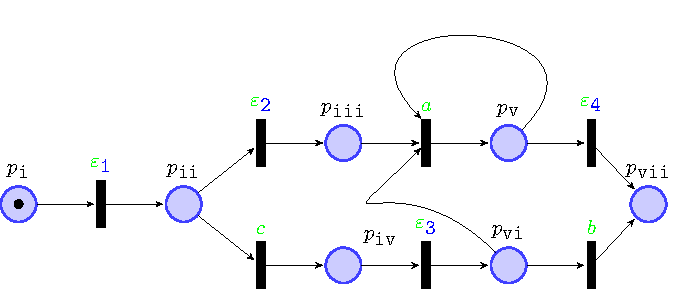
\includegraphics[width=.7\textwidth]{images/petri.pdf}
		\caption{A sample \uswn. Labels are shown in green, $\tau$ transitions in grey, weights in magenta.}\label{fig:spn}
	\end{minipage}\hfill \begin{minipage}{.49\textwidth}\centering
		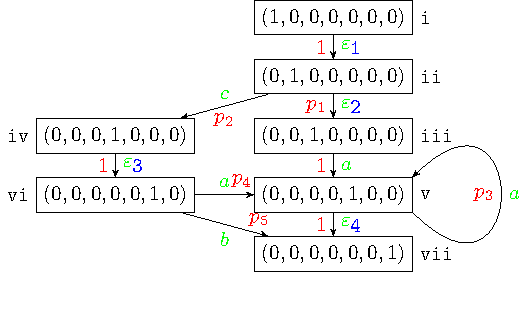
\includegraphics[width=.8\textwidth]{images/rg.pdf}
		\caption{Reachability graph $RG(N)$ of the \uswn $N$. Probabilities are shown in violet.}\label{fig:rg}
	\end{minipage}
\end{figure*} \begin{figure*}[!t]
	\begin{minipage}{.49\textwidth}\centering 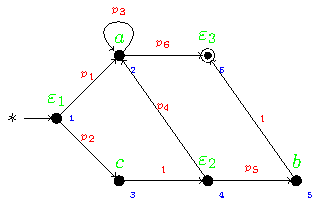
\includegraphics[width=.55\textwidth]{images/running_example.pdf}
	\caption{Transition graph $G_{RG(N)}$ encoding the reachability graph $RG(N)$.}\label{fig:lmc}\label{fig:orig}
\end{minipage}\hfill \begin{minipage}{.49\textwidth}\centering 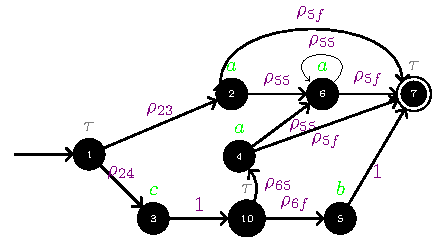
\includegraphics[width=.55\textwidth]{images/closed_example.pdf}
	\caption{Transition graph $\closed{G_{RG(N)}}$ resulting from the transition graph in $G_{RG(N)}$ after $\tau$-closure.}\label{fig:closed}
\end{minipage}
\end{figure*}


%Figures \ref{fig:spn} and \ref{fig:rg} respectively show a sample \uswn and its corresponding reachability graph. This net will be our running example throughout the paper.


%\begin{example}
%Figure \ref{fig:spn} provides a sample \uswn defined as such, and \ref{fig:rg} provides its associated Reachability Graph. This representation can be beneficial when such \uswns are inferred and extracted from log files \cite{PPNFromLog} for extracting the set of the probabilistic traces associated to the \uswn.
%\end{example}
%
%
%We use \uswns for modelling business processes: in fact, it can be shown \cite{RaedtsPUWGS07} that it is always possible to convert BPMNs to \uswns. Last, we also assume that a transition is enabled when all of its input places contain at least one token and that, when a transition fires, we remove one token from each of its input places and depose tokens for each of its output places.

We can show that there exists a conversion from $\rg{\net}$ (\figurename~\ref{fig:rg}) into a transition graph $\tg_{\rg{\net}}$ (\figurename~\ref{fig:orig}) preserving model traces as well as their probabilities via well-known techniques used to \emph{shift labels} from automata theory.  


\textbf{$\tau$-closure} The resulting transition graph $\tg_{\rg{\net}}$ is processed applying a \emph{$\hidden$-closure} that compiles away
$\tau$-transitions. This results into a new transition graph $\closed{\tg_{\rg{\net}}}$ (\figurename~\ref{fig:closed}) %that on the one hand only retains
retaining $\hidden$ labels only in the initial and accepting states while, for the rest, it exclusively operates over visible labels in $\tasks$. %, and, on the other, continues to preserve model traces and their probabilities. Also in this case we omit the details, as 
The transformation relies on well-known automata-based techniques for removing $\epsilon$-moves while preserving model traces, as well as their associated probabilities. %The only non-trivial observation is that, even in our case where probabilities are present, 
All $\tau$ transitions can still be removed thanks to the working hypothesis done for \uswn{s}, as no loops can contain only $\tau$ transitions. %The transition graph in \figurename~\ref{fig:orig} results in that of \figurename~\ref{fig:closed}.
\medskip

\textbf{Unfolding.} Next, we efficiently unfold the previously closed graph to collect TG-traces having probability greater or equal than $\pmin$ (\textsf{Minimum trace probability}) via the Eigen3 linear algebra library. Unfolding is efficiently performed via sparse matrices for TGs over the Eigen library. %The $\hidden$-closed transition graph $\closed{\tg_{\rg{\net}}}$ is \unravelled, so as to collect all the model traces that have a probability of at least $\pmin$. To do so, we rely on a key property that $\closed{\tg_{\rg{\net}}}$ inherits from the fact that it results from an \uswn. 
Since an \uswn has a Workflow net as underlying control-flow structure and given that TG inherits the results from SWNs, no loop can be executed without strictly decreasing the resulting probability. So, all valid sequences with a resulting probability of at least $\pmin$ can be enumerated and returned in a set. The so-obtained sequences are then combined by merging those that produce the same trace, summing up their probabilities, thus obtaining the set of all the traces having a probability greater than or equal to $\pmin$, $\ptraces{\closed{\tg_{\rg{\net}}}}{\pmin}$. The closure operation also implies that the notion of model trace collapses with the one of run modulo removing the initial and the final $\tau$ labels attached to the initial and accepting nodes. %In addition to that, traces might be also pre-filtered by \textsf{Maximum complete trace length}. 
\medskip

% !TeX root=../main.tex
\begin{figure}[!t]
	\hspace*{-1cm}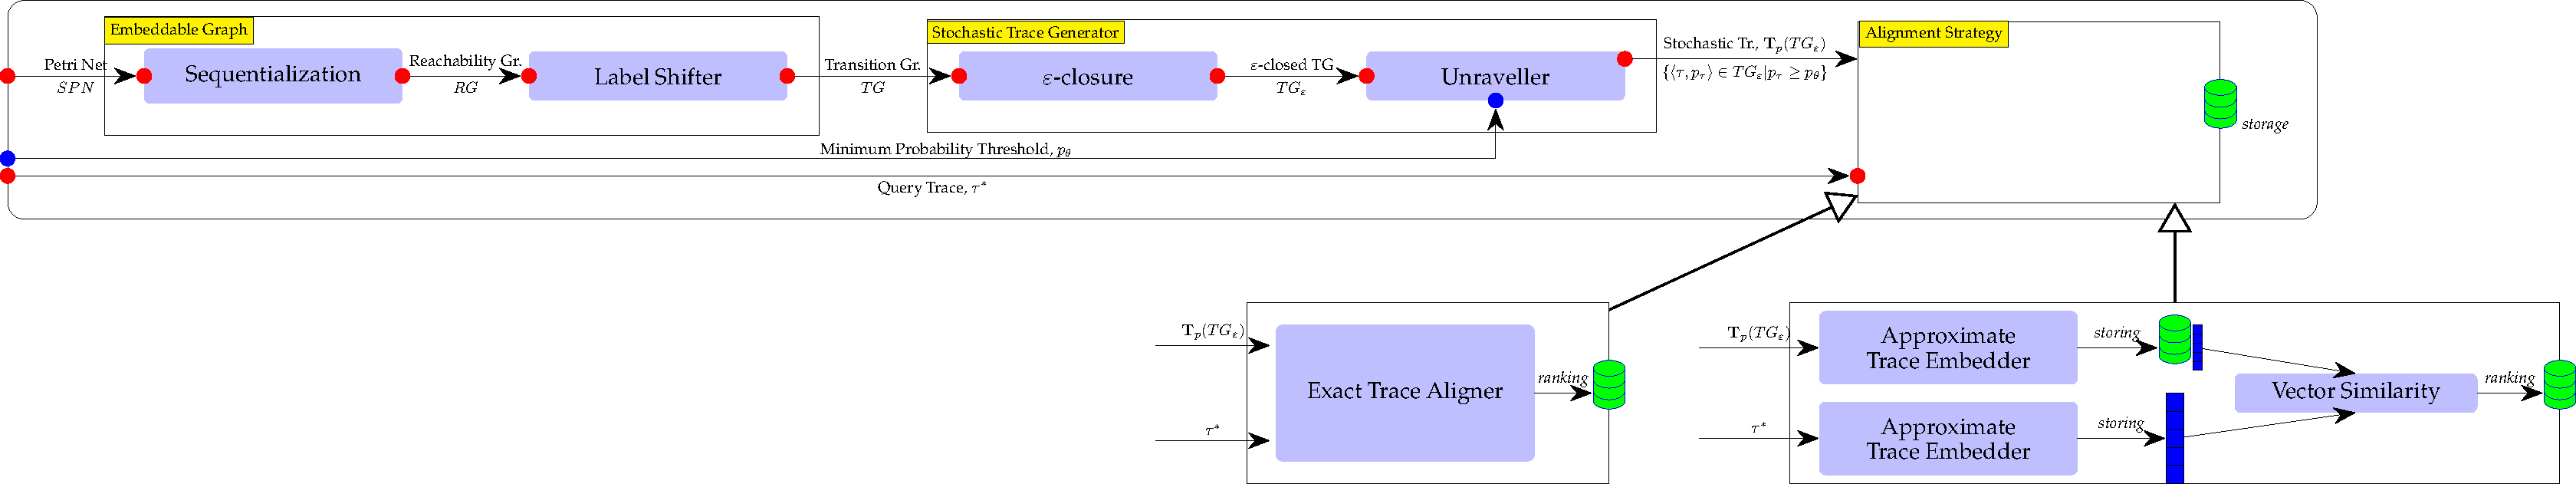
\includegraphics[width=1.2\textwidth]{images/pipeline}
	\caption{Proposed pipeline to assess the Probabilistic Trace Alignment}\label{fig:pipe}
\end{figure}


\section{Probabilistic Trace Alignment Pipeline}
We propose the pipeline from Figure \ref{fig:pipe} connecting several existing formalizations via intermediate processing steps.
The input of this pipeline is a query trace to be aligned, an \uswn, and a minimum probability threshold $\pmin$. Its output
is a set of model traces satisfying $\pmin$ with an alignment ranking.
%
The pipeline has the following phases: after representing the \uswn as a graph of all the sequentially scheduled transitions
(\S\ref{sec:seqZ}), we shift the labels from the edges towards the nodes while preserving the set of probabilistic traces
(\S\ref{sec:LSift}) and minimize the graph representation by removing the $\tau$-labelled nodes while preserving the
trace probability (\S\ref{sec:clos}). We extract the set of all traces having probability above $\pmin$ threshold (\S\ref{sec:unrav}) and  apply two different alignment strategies; one exact  (\S\ref{subsec:eta}), and one approximated.


We later discuss how to rank traces in the exact and approximated scenarios by reducing the alignment process to a k-nearest
neighbor problem. While the exact trace alignment requires to perform the alignment process each time a novel trace $\sigma^*$ is
introduced (\S\ref{subsec:exbkptap}), the approximated alignment can split the alignment into a preliminary loading phase and a
query phase. In the former, each stochastic trace from the \uswn is represented as a vector (\S\ref{subsec:ate}), and in the latter the to-be-aligned trace $\sigma^*$ is first represented as a vector and then compared to all the other vectorial representations.

\subsection{Sequentialization}\label{sec:seqZ}
The sequentialization step transforms an \uswn with an initial marking $M$ into a Reachability Graph $(\mathcal{M},\mathcal{E})$
generated by a sequentialization process, where potentially concurrent firing transitions are represented via a sequential scheduling.

\begin{definition}[Reachability Graph]
	Given an initial marking $M$ for an \uswn $\mathcal{U}$,  the \textit{Reachability Graph} for $\mathcal{U}$ is a graph
	$(\mathcal{M},\mathcal{E})$ where the nodes  $\mathcal{M}$ are composed of all the reachable markings from $M$,
	and the edges $\mathcal{E}$ are induced by the aforementioned relation $M\overset{t}{\to}M'$ among the
	nodes. To each edge $M\overset{t}{\to}M'$, we associate a transition probability $\mathbb{P}\left(M\overset{t}{\to}M'\right)=\frac{W(t)}{\sum_{t'\in E(M)}W(t')}$ \cite{spdwe}.
\end{definition}

\begin{example}
From the \uswn in Figure \ref{fig:spn}, the sequentialization process generates the reachability graph depicted in
Figure \ref{fig:rg}. Each node represents a marking $M$ as a vector, and the edges are labelled with the firing transitions.
The edges associated to this graph describe potentially concurrent firing transitions sequentially. While visiting the graph from
$M$, the chaining of the edge labels generates a trace produced from the untimed Workflow Net, and the product of the edge
weights provides the probability associated to the trace.
\end{example}



\subsection{Label Shifter}\label{sec:LSift}
Reachability graphs obtained via sequentialization cannot be directly embedded using existing methods:  Reachability graphs
associated to stochastic workflow nets are edge labelled, but TGs are node labelled. To represent the former as the latter, we
shift the labels from the edges to the nodes  while preserving the set of traces and their associated probability.
Such transformation is defined next.

\begin{definition}[Label Shifter]\label{def:transf}
The reachability graph $(\mathcal{M},\mathcal{E})$ generated from an initial marking $M$, is transformed into the TG $(s,t,L,R,1)$, where:
\begin{itemize}
	\item If is a single edge $M_1\overset{t}{\to}M_2\in\mathcal{E}$ where $M_1=M$, then $s=M\overset{t}{\to}M_2$; otherwise, define a new node $\textbf{i}$ and set it as the initial node for TG: $s=\textbf{i}$.
	\item If is a single edge $M_1\overset{t}{\to}M_2\in\mathcal{E}$ without outgoing edges in the reachability graph, then $t=M_1\overset{t}{\to}M_2$; otherwise, define a new node $\textbf{f}$ and set it as the accepting node for TG:  $t=\textbf{f}$.
	\item $[L]_{\lambda(t),\;M\overset{t}{\to} M'}=1$ for each $M\overset{t}{\to} M'\in\mathcal{E}$; if $\textbf{i}$ is defined then $[L]_{\tau\textbf{i}}=1$; if $\textbf{f}$ is defined, then $[L]_{\tau\textbf{f}}=1$; $[L]_{ij}=0$ otherwise.
	\item $[R]_{M\overset{t}{\to} M',\;M'\overset{t'}{\to} M''}=\frac{W(t')}{\sum_{\textbf{t}\in E(M')}W(\textbf{t})}$ for each $M\overset{t}{\to} M',M'\overset{t'}{\to} M''\in\mathcal{E}$; if $\textbf{i}$ is defined, $[R]_{\textbf{i},\;M\overset{t}{\to}M'}=\frac{W(t)}{\sum_{\textbf{t}\in E(M)}W(\textbf{t})}$; if $\textbf{f}$ is defined, then $[R]_{M\overset{t}{\to}M',\;\textbf{i}}=1$ for each $M'$ without outgoing edges in the reachability graph; $[R]_{ij}=0$ ow.
\end{itemize}
\end{definition}

\endinput
%
We can show that the TG obtained in Definition \ref{def:transf} preserves the same set of probabilistic traces associated by the reachability graph. The proof is omitted due to the lack of space.

\begin{example}
Figure \ref{fig:lmc} shows the TG obtained from the reachability graph in Figure \ref{fig:rg}. Nodes are labelled with the firing
transition labels (in green), and edges preserve the probabilistic information from the reachability graph (in red). Intuitively, when a
new initial node \textit{\textbf{i}} is inserted, we preserve all the initial probabilistic choices that a transition is fired from an initial
marking $M$, while the intermediate edges inherit the probabilisitc choice of the firing transition from the subsequent choices. When
a new final node \textit{\textbf{f}} is added, such edges always have probability $1$, and thus do not interfere with the
initial traces' probability.
\end{example}

\subsection{$\tau$-closure}\label{sec:clos}
The $\tau$-closure process has two main purposes: first, reduce the size of the previously generated TG by removing all
$\tau$-labelled nodes \texttt{\color{blue}w} and preserving the connection between  the nodes \texttt{\color{blue}u}
from its ingoing edges   $\texttt{\color{blue}u}\xrightarrow{\color{violet}\rho}\texttt{\color{blue}w}$ with the nodes \texttt{\color{blue}v} from its ingoing edges   $\texttt{\color{blue}w}\xrightarrow{\color{violet}\rho'}\texttt{\color{blue}v}$ by establishing new edges $\texttt{\color{blue}u}\xrightarrow{\color{violet}\rho\rho'}\texttt{\color{blue}v}$. $\tau$-labelled initial (or accepting) nodes are removed iff they have only one outgoing (ingoing) edge with probability $1$.

\begin{example}\todo{Is it now ok?}
	The $\tau$-closure removes the non-initial and non-accepting nodes within an automaton, while preserving the probabilistic trace equivalence of the two automata. Let us suppose to apply the $\tau$-closure to the automata in Figure \ref{fig:orig}: node \texttt{\color{blue}10} is removed alongside its associated edges, and new edges $\texttt{\color{blue}3}\xrightarrow{\color{violet}\rho_{65}}\texttt{\color{blue}4}$ and $\texttt{\color{blue}3}\xrightarrow{\color{violet}\rho_{6f}}\texttt{\color{blue}5}$ are introduced. The resulting TG $P$ is represented with the same graphical depiction Figure \ref{fig:closed}.
\end{example}
%
Consequently, it is always possible to minimize a TG  via $\tau$-closure, so that the only nodes labelled as $\tau$
are the source and the target nodes and the set of weighted traces is preserved. From now on, we consider only minimised TGs.

\subsection{Unraveller}\label{sec:unrav}
%Being that both the graph isomorphism problem is NP-Complete and the
Since TGs are fully characterized by the set of the probabilistic traces that they generate,  we say that two TGs are
(probabilistic-trace) equivalent iff they share the same set of weighted traces. In particular, we denote as $\mathcal{W}_p^n(P)$ the set of all the weighted traces in $P$ having at least probability $p$ and maximum length $n$. Under these assumptions, the probabilistic trace equivalence is deterministic.

\begin{example}
	The set $\mathcal{W}_0^{\aleph_0}(P^*)$ of weighted traces of the TG in Figure \ref{fig:orig} is
%	The TG in Figure \ref{fig:orig} has the following set $\mathcal{W}_0^{\aleph_0}(P^*)$ of weighted traces:
$$\set{\braket{\underbrace{\color{green}a\dots a}_{n},{\color{violet}\pa\pc^n\pf}}|n\in \mathbb{N}_{>0}}\cup \set{\braket{{\color{green}c}\underbrace{\color{green}a\dots a}_{n},{\color{violet}\pb\pd\pc^n\pf}}|n\in \mathbb{N}_{>0}}\cup\{\braket{{\color{green}cb},{\color{violet}\pb\pe}}\}$$
After the $\tau$-closure process, $\mathcal{W}_0^{\aleph_0}(P^*)=\mathcal{W}_0^{\aleph_0}(P)$, so the two TGs are (probabilistic-trace) equivalent.
\end{example}

\section{Top-k Trace Alignment}\label{sec:topk}
Trace alignments algorithms provide as output a single alignment. This is not very convenient in practice because a rich feedback should provide different possibilities. This is even more important when the Workflow Nets (such as USWNs) are stochastic and the different model traces have different probabilities. {Instead, we would like to return the best $k$ alignments among all the possible unravelled traces from the USWN $\mathcal{U}$. If we want to return the best $k$ alignments from $\mathcal{U}$ for a trace $\tau^*$, the approach descrived in the previous section requires to visit the entire search space $\mathcal{W}_{p_\theta}^n(P)$ where $P$ is the TG associated to $\mathcal{U}$. On the other hand, we prefer to reduce the search space by starting the visit from the traces nearer to $\tau^*$.}


%\texttt{\color{red}[TODO: introduction, motivation, and why it is useful to run it as a $k$-best search]}
%\resizeableyellownote{3}{3}{
%	Assuming that Rafael writes the definition of his ranking function, that can be expressed as $r(\tau^*,\tau)=d(\tau^*,\tau)w_\tau$ for a query trace $\tau^*$ and a trace $\tau\in\mathcal{W}_p^n(P)$
%}

$k$-nearest neighbours ($k$NN) is a well-known problem in database theory \cite{Altman} which has the goal of finding the $k$ nearest data points to a query $x$ from a set $\mathcal{X}$ of data points via a distance function $d$ defined over $\mathcal{X}\cup\{x\}$. {If the query  $x$ is performed over ad-hoc data structures (Vp-Trees \cite{Fu2000}, Kd-Trees \cite{Maneewongvatana99}, and M-Trees \cite{Ciaccia}), then we can start our search straight from the nearest neighbours of $x$ in $\mathcal{X}$ by preordering  $\mathcal{X}$ within the data structure of choice via $d$. This characterization could be exploited for top-$k$ trace alignments: if $x$ is the trace $\tau^*$ that we want to align over the unravelled traces $\mathcal{X}=\mathcal{W}^n_{p_\theta}(P)$ and $d$ is correlated to the alignment cost for probabilistic traces, then $k$-nearest neighbours describes the best $k$ alignments for  $\tau^*$.}
	
{For the aforementioned data structures, 
$x$ (and $\mathcal{X}$) is usually represented as a (set of) vector(s) via embedding  $\phi$, while the distance $d$ can be either the Euclidean distance or an ad-hoc vector distance $d_{k_\phi}$ defined over $k_\phi$ (see Equation \ref{eq:dofk}). $\phi$ is chosen to be independent from the query $x$, so that all the vectors $\phi(x_i)$ for $x_i\in\mathcal{X}$ are not changed for each new query $x$.}

\begin{figure}[!t]
	\centering
	\subfloat[The similarity/probability space.]{\label{fig:spp}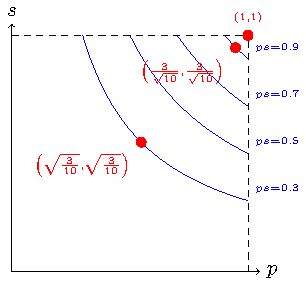
\includegraphics[width=.45\textwidth]{images/original_space.pdf}}\qquad
	\subfloat[The transformed space for the $k$ nearest neighbours problem.]{\label{fig:knnspace}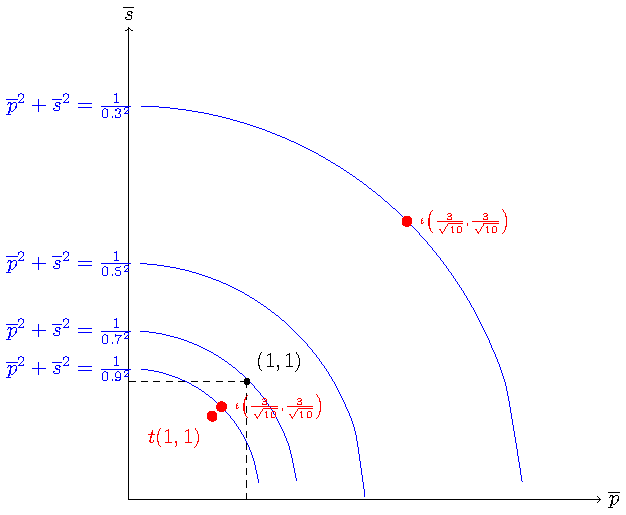
\includegraphics[scale=0.55]{images/transformed_space.pdf}}\\
	\caption{Two different characterizations of the probabilistic trace alignment problem. The best possible match is represented in red in both the similarity/probability space and in the transformed one.}
\end{figure}
\ADD{Concerning the approximate-ranking trace embedder, it} meets the $k$NN desiderata as $\phi_{\mathcal{P}}$ is defined independently from $\tau^*$: \ADD{by exploiting the aforementioned data structures, it implies that we can retrieve the top-$1$ alignment according to $k_{\mathcal{P}}$ by traversing the preloaded data structure at most with an initial logarithmic look-up search, from which we can visit the surrounding search space for retriev-\\ing the remaining $k-1$ traces. On the other hand, the}  $k_\star$ \ADD{associated to the  optimal-\\ranking trace aligner } is tightly bounded to the specific $\tau^*$ of choice via the alignment cost $d$, \ADD{thus implying that computing the embedding for the top-$1$ trace requires a preliminary linear visit of all the traces in $\mathcal{X}$} In order to maximise the decoupling of the vectorial representation from $\tau^*$ with $w_{\tau^*}=1$, 
 we propose 
 to embed each unravelled trace $\braket{\tau,w_\tau}$ via $\phi_\star(\braket{\tau,w_\tau})=\Big(\frac{1}{w_\tau\sqrt{w_\tau^2+s_d^2(\tau,\tau^*)}},$\\  $\frac{1}{s_d(\tau,\tau^*)\sqrt{w_\tau^2+s_d^2(\tau,\tau^*)}}\Big)$ (Figure \ref{fig:knnspace}) and the to-be-aligned trace $\tau^*$ to $x=(0,0)$, so that the the Euclidean distance between the vector of an unravelled trace in $\mathcal{X}$ and the origin $x$ is  inversely proportional to $k_\star(\tau,\tau^*)$. The proof is omitted due to lack of space. \ADD{Thus, $k_\star$ requires to always pay a linear scanning cost for each new trace $\sigma$ that we want to align before the logarithmic cost of the top-$1$ lookup in the transformed space (Figure \ref{fig:knnspace}).}
 
\begin{example}
	Figure \ref{fig:spp} shows a family of hyperbolae $w_\tau s(\tau,\tau^*)=k$ describing all the points $(w_\tau, s(\tau,\tau^*))$ having $k$ as a $k_\star$ score. Point $\color{red}(1,1)$ represents the best possible trace match, as it means that there exists a trace $\braket{\tau,w_\tau}\in\mathcal{W}_{p_\theta}^n(P)$ where $\tau=\tau^*$ and $w_\tau=1$.
		Figure \ref{fig:knnspace} shows that the aforementioned embedding moves the points of the hyperbola $w_\tau s(\tau,\tau^*)=k$ over a circumference $x^2+y^2=\sfrac{1}{k^2}$ describing a locus of the points equidistant from the origin of the axes $(0,0)$ with distance $\sfrac{1}{k}$: this intuitively means that the $k$NN algorithm will first visit the points nearer to the origin by picking up the nearest circumference first, and then will visit the next circumference.
\end{example}

%\xout{In particular, we want to exploit the well-known \textit{k}-nearest neighbour problem for providing this desired result. Such problem can be formalized as follows:}
%\begin{definition}[$k$-Nearest Neighbour]
%	\xout{Given a set of vectors  $\mathcal{X}\subseteq \mathbb{R}^d$ within a $d$-dimensional Euclidean space and a query vector $q\in\mathbb{R}^d$, the $k$-nearest neighbour algorithm returns a subset $K\subseteq\mathcal{X}$ of $k$ elements minimizing the distance from $v$:}
%	$$\Rcancel{knn_\delta(k,q,\mathcal{X})=\begin{cases}
%	\emptyset& k \leq 0\\
%	\{c\}\cup knn(k-1,q,\mathcal{X}\backslash\{c\}) & k> 0 \Rightarrow c:={\arg\min}_{x\in\mathcal{X}}\delta(x,q)\\
%	\end{cases}}$$
%	\xout{where $\delta$ is a distance measure between the vectors.}
%\end{definition}
%{While for the proposed approximate trace embedder we can directly use this formulation by exploiting an embedding $\phi_{\mathcal{P}}$ and a distance $d(\tau,{\tau^*})=1-k_{\phi_\mathcal{P}}(P_\tau,P_{\tau^*})$ \xout{for $k_{\phi_\mathcal{P}}(P,P')$ returns $1$ as a maximum value}, the price that we need to pay if we want to exploit the existing aligners is alignment cost for all the unravelled traces in $\mathcal{X}$. In fact, we can either directly exploit $k_\star$ and the fact that kernels can be always expressed as distance functions $d_{k_\star}$ \cite{Gartner03}, or we need to transform each unravelled trace $\braket{\tau,w_\tau}$ as a point $(x,y)\in\mathbb{R}_{\geq 0}^2$ and the to-be-aligned trace $\tau^*$ as an arbitrary vector $(0,0)$, so that the Euclidean distance between the two associated vectors is proportional to $d_{k_\star}$. Given that the ordering of the traces depends on trace to be aligned, this implies to either re-sort the data all the time or to re-compute the associated embedding from scratch.}
%
%\subsection{Exact $k$-probabilistic Traces Alignment Problem}\label{subsec:exbkptap}
%%\texttt{\color{red}[TODO: the introduction of this section depends on how we want to formulate the problem. I suddenly start with the definition of the k-Nearest Neighbour, but I am aware that we need to provide first a bit of context]}
%
%
%
%\xout{In order to reduce the exact probabilistic trace alignment problem to the \textit{k}-nearest neighbour, we can first map each weighted trace  $\braket{\tau,w_\tau}\in\mathcal{W}_p^n(P)$ that we need to align with $\tau^*$ as a point $\tau\overset{\mu_{\tau^*}}{\mapsto}(w_\tau,\; s_d(\tau,\tau^*))$ in the 2-dimensional similarity/probability space of coordinates $(p,s)$, so that the trace finding problem reduces to find a data point maximising the product $p\cdot s\equiv w_\tau\cdot s_d(\tau,\tau^*)$ (Figure \ref{fig:spp}).}
%
%%\begin{table}[!t]
%%\centering
%%\caption{Expected ranking of the paths from Example \ref{ex:withpaths} with the trace $\tau^*=\textup{caba}$. The cost function is the one from \cite{LeoniM17} and its normalized similarity score has $c=5$.}\label{tab:expected}
%%\begin{tabular}{lc|ll|cl}
%%	\toprule
%%	
%%	\multirow{2}{*}{$\tau$} &
%%	\multirow{2}{*}{$d(\tau,\tau^*)$} &
%%	\multicolumn{2}{c|}{$\mu_{\tau^*}$} &
%%	 \multirow{2}{*}{$\approx s_d(\tau,\tau^*)\cdot w_\tau$} & \multirow{2}{*}{\textit{expected ranking}}\\
%%	
%%	\cline{3-4} &&  $\langle w_\tau$ &  $,\,s_d(\tau,\tau^*)\rangle $ &&\\
%%	
%%	\midrule
%%	{a}  & $3$ & $0.4$ & $\;\; 0.6250$  & $0.2500$ & \textbf{1}\\
%%	{aa}  & $2$ & $0.2$ & $\;\; 0.7142$ & $0.1428$ & \textbf{2}\\
%%	{aaa}  & $2$ & $0.1$ & $\;\; 0.7142$ & $0.0714$ & \textbf{3}\\
%%	{ca}  & $2$ & $0.07$ & $\;\; 0.7142$ & $0.0500$ & \textbf{4}\\
%%	{cb}  & $2$ & $0.06$ & $\;\; 0.7142$ & $0.0428$ & \textbf{5}\\
%%	{aaaa}  & $3$ & $0.05$ & $\;\; 0.7142$ & $0.0357$ & \textbf{6}\\
%%	{caa}  & $1$ & $0.035$ & $\;\; 0.8333$ & $0.0292$ &  \textbf{7}\\
%%	{caaa}  & $1$  & $0.0175$ & $\;\; 0.8333$ & $0.0145$ & \textbf{8}\\
%%	\bottomrule
%%\end{tabular}
%%\end{table}
%\begin{example}\label{ex:rankingTaus}
%\xout{Table \ref{tab:expected} represents the expected exact alignment raking of all the weighted traces $\braket{\tau,w_\tau}\in\mathcal{W}_0^4(P)$ generated by the TG $P$ in Figure \ref{3figs} with a trace $\tau^*=\textup{caba}$.  Albeit traces \textit{caa} and \textit{caaa} are the most similar with \textit{caba}, their associated trace probability is $w_\tau$ is rather low, so traces having higher probability but lower similarity score are preferred (e.g., \textit{a} and \textit{aa}). Given that users might still prefer the most similar ones to the ones maximising both probability and similarity, we prefer to offer the user the whole set of the best $k$ solutions rather than cherry-picking the best solution maximising both probability and similarity.}
%\end{example}
%
%\xout{After this preliminary step, we can finall reduce the problem into the desired $k$-nearest neighbour by exploiting $\delta$ as the usual Euclidean Distance. In order to do so, we define a transformation $t$ such that the distance of $t(p,s)$ towards  the origin of the axes $\vec{0}$ (representing the trace to be aligned $\tau^*$) corresponds to $\sfrac{1}{ps}$, so the transformed data points maximising $ps=k$ are all at the same distance $\sfrac{1}{k}$ from $\vec{0}$ (Figure \ref{fig:knnspace}). A possible transformation is the following:}
%\[t(p,s):=\left(\frac{1}{s\sqrt{p^2+s^2}},\; \frac{1}{p\sqrt{p^2+s^2}}\right)\]
%
%
%
%
%
%
% \xout{We can show with the next lemma that the following transformation is the one reducing the problem to the $k$-Nearest Neighbour problem:}
%
%
%
%\begin{lemma}
%\xout{Given a value $k\in[0,1]\subseteq \mathbb{R}^+_0$, the set of points having the product $ps$ at least $k$ corresponts to the set of $t$-transformed points having a distance of at least $1/k$ from the origin of the axes.}
%\end{lemma}
%\begin{proof}
%\[\begin{aligned}
%ps\geq k&\Rcancel{\Leftrightarrow \frac{1}{ps}\leq\frac{1}{k}} \\
%	   &\Rcancel{\Leftrightarrow \frac{\sqrt{p^2+s^2}}{ps\sqrt{p^2+s^2}}\leq\frac{1}{k} }\\
%	   &\Rcancel{\Leftrightarrow \sqrt{\frac{p^2+s^2}{p^2s^2(p^2+s^2)}}\leq\frac{1}{k}} \\
%	   &\Rcancel{\Leftrightarrow \sqrt{\frac{p^2}{p^2s^2(p^2+s^2)}+\frac{s^2}{p^2s^2(p^2+s^2)}}\leq\frac{1}{k}} \\
%	   &\Rcancel{\Leftrightarrow \sqrt{\frac{1}{s^2(p^2+s^2)}+\frac{1}{p^2(p^2+s^2)}}\leq\frac{1}{k}} \\
%	   &\Rcancel{\Leftrightarrow \left\|{\biggr({\frac{1}{s\sqrt{p^2+s^2}},\frac{1}{p\sqrt{p^2+s^2}}\biggr)}-\vec{0}}\right\|_2\leq\frac{1}{k}} \\
%	   &\Rcancel{\Leftrightarrow \left\|t(p,s)-\vec{0}\right\|_2\leq\frac{1}{k}} \\
%\end{aligned}\]
%\end{proof}
%\begin{lemma}
%\xout{Given a Workflow Net $P$ and a trace $t^*$, the probabilistic trace alignment problem of the best $k$ traces reduces to the $k$-Nearest Neighbour problem $\mu_{\tau^*}^{-1}(knn(k,\vec{0},\mu_{\tau^*}(\mathcal{W}_0^{\aleph_0}(P))))$.}
%\end{lemma}
%\begin{proof}
%\xout{Trivial by definition of $\mu_{\tau^*}$ and for the previous lemma.}
%\end{proof}
%
%%\begin{table}[!t]
%%\centering
%%\caption{Representing the point from Table \ref{tab:expected} in the transformed space.}\label{tab:transf}
%%\begin{tabular}{ll|lll}
%%	\toprule
%%	
%%	$\tau$ & $t(\mu_{\tau^*}(\tau))$ & $\norm{t(\mu_{\tau^*}(\tau))-\vec{0}}{2}$ & $\frac{1}{\norm{t(\mu_{\tau^*}(\tau))-\vec{0}}{2}}$ & \textit{distance ranking}\\
%%	
%%	\midrule	
%%	a   & $\braket{2.16, \;\,3.37}$ & $4.00$ & $0.2500$ & \textbf{1}\\
%%	{aa}  & $\braket{1.89, \;\,6.74}$ & $7.00$ & $0.1428$ & \textbf{2}\\
%%	aaa   & $\braket{1.94, 13.87}$ & $14.00$ & $0.0714$ & \textbf{3}\\
%%	ca   & $\braket{1.95, 19.91}$ & $20$ & $0.0500$ & \textbf{4}\\
%%	{cb}  & $\braket{1.95, 23.25}$ & $23.33$ & $0.0428$ & \textbf{5}\\
%%aaaa   & $\braket{1.95, 27.93}$ & $28.00$ & $0.0357$ & \textbf{6}\\
%%caa   & $\braket{1.44, 34.26}$ & $34.29$ & $0.0292$ & \textbf{7}\\
%%caaa   & $\braket{1.44, 68.56}$ & $68.57$ & $0.0145$ & \textbf{8}\\
%%	\bottomrule
%%\end{tabular}
%%\end{table}
%\begin{example}
%\xout{We now want to show the correctness of the former lemmas with some examples.
%Table \ref{tab:transf} represents the transformed points $t(\mu_{\tau^*}(\tau))$ from the data points $\mu_{\tau^*}(\tau)$  calculated  Example \ref{ex:rankingTaus}. The third column shows the distance of the transformed point from the origin: the following column shows that the inverse of such distance exactly represents the previously calculated $s_d(\tau,\tau^*)\cdot w_\tau$, thus empirically implying that the $k$-nearest neighbours problem corresponts to the best $k$ traces maximising the product $s_d(\tau,\tau^*)\cdot w_\tau$.}
%\end{example}
%
%
%
%
%
%\xout{At this stage, we can solve the $k$-probabilistic trace alignment problem by generating a new instance of the $k$-Nearest Neighbour problem for each possible trace $\tau^*$ that we want to align towards the traces coming from a TG. On the other hand, this solution might result quite costly, as solving the problem would require either to use a brute force search algorithm or to load and index our set of points each time.\yellownote{TODO: add references and explanation to the problem (we need a Related Work section\dots? I am accustomed to write such sections.)} In the next section we will discuss an approximated version of the problem providing a trade-off between accuracy and efficiency.}
%
%
%\subsection{Approximate $k$-probabilistic Traces Alignment Problem}\label{subsec:akptap}
%\xout{Given that in the approximated characterization the traces are immediately represented as vectors, we can observe that the approximate $k$-probabilistic Trace Alignment Problem can be characterized as $knn_d(k,\phi(\tau^*),\phi(\mathcal{W}_{p_\theta}(P)))$, where $d(u,v)$ is defined as the inverse of the normalized dot product, i.e. $d(u,v)=1-\frac{\braket{u,v}}{\sqrt{\braket{u,u}\braket{v,v}}}$. }
%
%
%
%\textit{Trace alignments algorithms provide as output a single alignment. This is not very convenient in practice because a rich feedback should provide different possibilities. This is even more important when the Workflow Net we are considering is stochastic and the different model traces have different probabilities.}
%
%\textit{INPUT: trace, stochastic (Workflow net) Workflow Net, minimum probability threshold, maximum model trace length
%OUTPUT: set of model traces satisfying the minimum probability threshold and the maximum model trace length candidates for the alignment with an alignment ranking}

\begin{table}[!t]
\caption{Distinct USWNs and associated sets of unravelled traces from a single Sepsis Cases Event Log \cite{mannhardt_2016}.}\label{tab:dataset}
 \begin{adjustbox}{max width=\textwidth}
	\begin{tabular}{crl||cl|c}
		\toprule
		\textbf{Experiment Conf.} $(\mathcal{U})$ & \textit{Model} & $+$\textit{W. Estimator} & $n$ & $p_\theta$& $\;\;|\mathcal{W}_{p_\theta}^n(P_{\mathcal{U}})|$ \\
		\midrule
		
		\textbf{SM\_CONS\_20} &SplitMiner 2.0  \cite{AugustoCDRP19}       & +\texttt{Constant} & $20$ & $\;\;0$ & $157$  \\
		
		\textbf{SM\_FORK\_20} & SplitMiner 2.0  \cite{AugustoCDRP19}      & +Fork \cite{spdwe} & $20$ & $\;\;0$ & $32$  \\
		
		
		\textbf{SM\_PAIR\_20} & SplitMiner 2.0  \cite{AugustoCDRP19}      & +PairScale \cite{spdwe} & $20$ & $\;\;0$ & $157$ \\
		
		\textbf{SM\_PETRI\_20} & \multicolumn{2}{c||}{Rogge-Solti \cite{RoggeSoltiAW13}} & $20$ & $10^{-5}$ & $1612$ \\
		\bottomrule
	\end{tabular}
\end{adjustbox}
\end{table}
\section{Experimental Results}\label{sec:exp}
\subsection{Dataset}
For our experiments, we took the Sepsis Cases Event Log \cite{mannhardt_2016}, splitted the dataset into the ``\textit{happy traces}'' occurring approximately near to the trace average length ($\leq 2.3\cdot 10^{7}$ ms), and used this dataset to generate either a USWN via ProM \cite{RoggeSoltiAW13} and a BPMN with only exclusive gates using Split Miner 2.0 \cite{AugustoCDRP19} that was then converted into a Petri Net \cite{PPNFromLog}. Such Petri Net was later on converted into a USWN by using a firing weight estimator: we choose the Fork and the PairScale estimators from \cite{spdwe} and we denote as \texttt{Constant} a naïve estimator assuming that each all the transition probabilities from a given marking are equiprobable. No estimator was used for the USWN generated via ProM, as such engine already estimates the firing weights. From such USWNs, we generate distinct sets of unravelled traces. All these steps are summarised in Table \ref{tab:dataset}. The following experiments have the aim of evaluating the benefits of performing the Approximate-Ranking strategy over the Optimal-Ranking one.

\begin{figure*}[!t]
\begin{minipage}{.49\textwidth}

	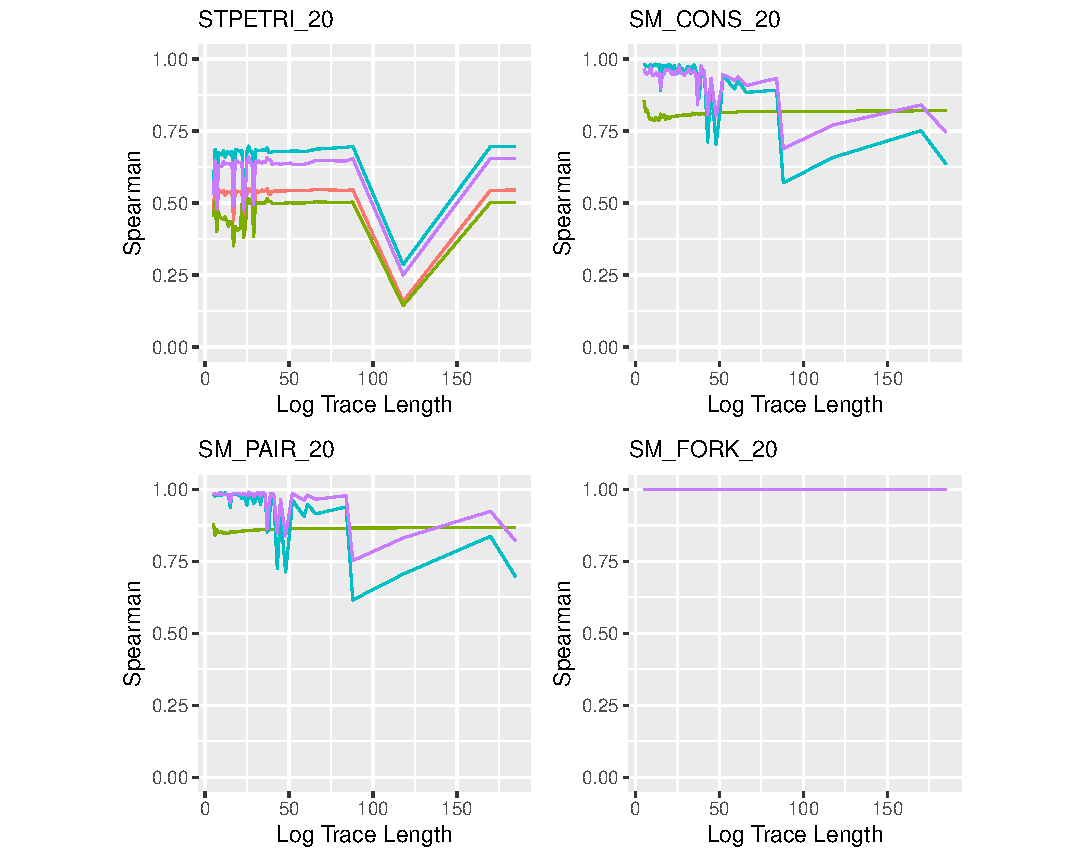
\includegraphics[width=1.1\textwidth]{images/Prec.pdf}
	\caption{Approximation comparison.}\label{fig:app}
\end{minipage}\hfill \begin{minipage}{.49\textwidth}

	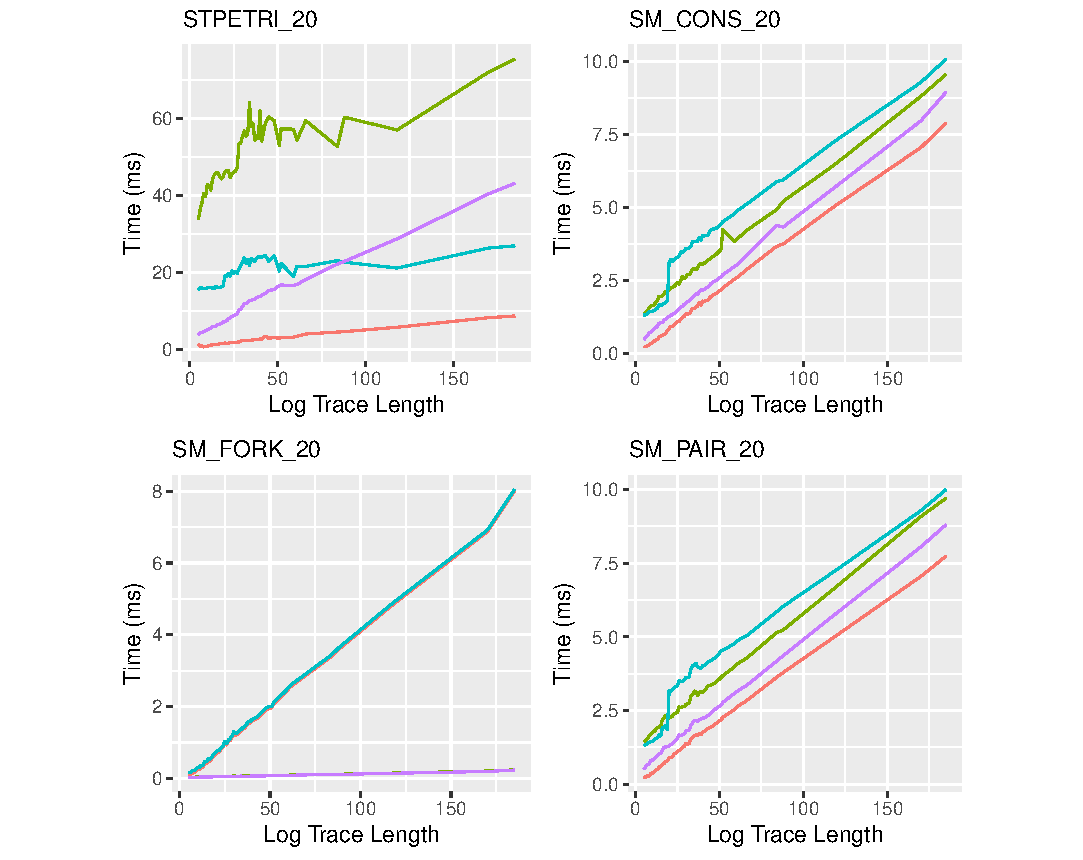
\includegraphics[width=1.1\textwidth]{images/kronos.pdf}
	\caption{$k$NN alignment benchmark.}\label{fig:kronos}
\end{minipage}
\end{figure*}
\subsection{Approximation}\label{subsec:apprp}
In order to assess how well the proposed Approximate-Ranking strategy approximates the Optimal-Ranking one, we use the Spearman Correlation Index \cite{} to express the correlation between each sub-embedding strategies for $\phi_{\mathcal{P}}$ ($\color{ggplotGreen}\epsilon^1\&\nu^1$, $\color{ggplotRed}\epsilon^2\&\nu^1$, $\color{ggplotPurple}\epsilon^1\&\nu^2$, and $\color{ggplotBlue}\epsilon^2\&\nu^2$) and the Optimal-Ranking one.
In general, we can see form the plots that when aligning longer traces, the correlation of the approximate rankings with the optimal one is lower. This is due to the fact that, in this case, the embedding representing the trace to align is longer and this implies also a larger approximation error. We can also observe that the sub-embeddings considering only information about the edges (i.e., the one where the features corresponding to the $\nu$ dimension are set to zero) have in general a higher correlation with the Optimal-Ranking strategy, but their correlation values are less stable with respect to the length of the trace to be aligned. In the case of \textbf{SM\_FORK\_20}, the correlation is maximum for all sub-embedding strategies.

%set of unravelled traces in Table \ref{tab:dataset} and the subset of the Sepsis Cases Event Log that was not used to generate the USWNs. For each of this log trace $\sigma^*$ we added controlled noise (transition addition, deletion, or swap) at either $20\%$ ($\tilde{\sigma}^*$) or $30\%$ ($\tilde{\tilde{{\sigma}}}^*$) of the log trace as for \cite{LeoniM17}. Then, we found the correlation between the ranking $R_\star$ induced by $k_{\phi_{\mathcal{P}}}(\sigma,\sigma^*)$ to the ranking induced by replacing $\sigma^*$ with one of the two noised traces (either a ranking $R_{20}$ induced by $k_{\phi_{\mathcal{P}}}(\sigma,\tilde{\sigma}^*)$ or $R_{30}$ induced by $k_{\phi_{\mathcal{P}}}(\sigma,\tilde{\tilde{\sigma}}^*)$). The correlation $\rho$ between these two rankings ($\rho(R_\star,R_{20})$ and $\rho(R_\star,R_{30})$) is performed via Spearman Correlation Index $\rho$: such index will return near-$1$ on increasing monotonic trend, near-$(-1)$ values on decreasing monotonic trend, and near-$0$ values where the two rankings are almost uncorrelated. Figure \ref{fig:app} shows the outcome of such experiments for all the possible combinations of $\epsilon$ and $\nu$ sub-embeddings for $\phi_{\mathcal{P}}$ while varying the log trace length. We can observe that strategies including traces' frequencies ($\nu^1$) are more stable if compared to strategies where such information is completely ignored ($\nu^2$). Furthermore, such approximation never reaches zero values, while that occurrence might happen for $\nu^2$-based strategies.

\subsection{Efficiency}\label{subsec:efficio}
With reference to the plots in Figure \ref{fig:kronos}, 
we evaluated the efficiency of computing the trace alignment over both Optimal- ({\color{ggplotPurple}Purple} and {\color{ggplotGreen}Green}) and Approximated-ranking ({\color{ggplotBlue}Blue} and {\color{ggplotRed}Red}) strategies over two different data structures enabling $k$NN queries, i.e., VP-Trees ({\color{ggplotBlue}Blue} and {\color{ggplotPurple}Purple}) and KD-Trees ({\color{ggplotRed}Red} and {\color{ggplotGreen}Green}). We conduct our experiments for $k=20$\ADD{, and we use the Levenshtein distance as a baseline distance for the alignment cost function}. While the query time for the Optimal-Ranking  includes the additional \textit{indexing time} for generating all the vectors to the neighbourhood search, the Approximated-Ranking  adds the neighbourhood search time with the embedding transformation of $x$; in particular, we consider the average embedding time for all the possible embedding strategies described in the previous experiment setting. Figure \ref{fig:kronos} plots the result of such experiments: the time required to generate and load all the $\phi_\star$ truly dominates the cost of generating the embedding $\phi_{\mathcal{P}}(x)$ for bigger datasets such as \textbf{STPETRI\_20}, while the cost for $\phi_{\mathcal{P}}(x)$ becomes non-negligible when we have just a few traces to align (\textbf{SM\_FORK\_20}). Last, while the $k$NN alignments over $\phi_{\mathcal{P}}$ always provide the best timing results via KD-Trees, we cannot elect a best data structure $\phi_\star$ that is valid for all datasets and all trace lengths. 
%\section{Conclusions}
%\texttt{\color{red}[TODO]}
%\label{sec:conclusion}
%
%We have studied how to enrich constraint-based process models with uncertainty, captured as the probability that a trace will conform with a constraint or not. We have discussed how this impacts the semantics of a constraint model, and how logical and probabilistic reasoning have to be combined to provide core services such as consistency and conformance checking, as well as probabilistic constraint entailment.
%
%Notably, all the techniques presented in this paper can be directly grounded with existing tools: automata-based techniques for \LTLf to carry out logical reasoning, and off-the-shelf systems to solve systems of linear inequalities (and corresponding optimization problems) to handle probabilities.
%
%In~\cite{DBLP:conf/bpm/Maggi2020}, beside a concrete implementation of the techniques presented in this paper, we investigate the application of probabilistic business constraints to process mining, not only considering standard problems like discovery, but also delving into online operational support and, in particular, probabilistic monitoring~\cite{DBLP:conf/fase/MaggiMA12}.

%Balancing between the likelihood of the model trace with respect to which we are computing the alignment and the cost of the alignment (if the cost of the alignment is too high even if the model trace is very likely applying too many changes in the original trace is in turn not very likely).

%\section*{Acknowledgements}


%This research has been partially supported by the project IDEE (FESR1133) funded by the Eur.\ Reg.\ Development Fund (ERDF) Investment for Growth and Jobs Programme 2014-2020. 


\bibliographystyle{splncs04}
\bibliography{biblio3}
%,bibliography2,references,libraryFiltered,main,Bibliography-CDC,DiCiccio,biblio}




\end{document}
